% Options for packages loaded elsewhere
\PassOptionsToPackage{unicode}{hyperref}
\PassOptionsToPackage{hyphens}{url}
%
\documentclass[
  11pt,
]{article}
\usepackage{lmodern}
\usepackage{amssymb,amsmath}
\usepackage{ifxetex,ifluatex}
\ifnum 0\ifxetex 1\fi\ifluatex 1\fi=0 % if pdftex
  \usepackage[T1]{fontenc}
  \usepackage[utf8]{inputenc}
  \usepackage{textcomp} % provide euro and other symbols
\else % if luatex or xetex
  \usepackage{unicode-math}
  \defaultfontfeatures{Scale=MatchLowercase}
  \defaultfontfeatures[\rmfamily]{Ligatures=TeX,Scale=1}
\fi
% Use upquote if available, for straight quotes in verbatim environments
\IfFileExists{upquote.sty}{\usepackage{upquote}}{}
\IfFileExists{microtype.sty}{% use microtype if available
  \usepackage[]{microtype}
  \UseMicrotypeSet[protrusion]{basicmath} % disable protrusion for tt fonts
}{}
\makeatletter
\@ifundefined{KOMAClassName}{% if non-KOMA class
  \IfFileExists{parskip.sty}{%
    \usepackage{parskip}
  }{% else
    \setlength{\parindent}{0pt}
    \setlength{\parskip}{6pt plus 2pt minus 1pt}}
}{% if KOMA class
  \KOMAoptions{parskip=half}}
\makeatother
\usepackage{xcolor}
\IfFileExists{xurl.sty}{\usepackage{xurl}}{} % add URL line breaks if available
\IfFileExists{bookmark.sty}{\usepackage{bookmark}}{\usepackage{hyperref}}
\hypersetup{
  hidelinks,
  pdfcreator={LaTeX via pandoc}}
\urlstyle{same} % disable monospaced font for URLs
\usepackage[margin=1.0in]{geometry}
\usepackage{graphicx,grffile}
\makeatletter
\def\maxwidth{\ifdim\Gin@nat@width>\linewidth\linewidth\else\Gin@nat@width\fi}
\def\maxheight{\ifdim\Gin@nat@height>\textheight\textheight\else\Gin@nat@height\fi}
\makeatother
% Scale images if necessary, so that they will not overflow the page
% margins by default, and it is still possible to overwrite the defaults
% using explicit options in \includegraphics[width, height, ...]{}
\setkeys{Gin}{width=\maxwidth,height=\maxheight,keepaspectratio}
% Set default figure placement to htbp
\makeatletter
\def\fps@figure{htbp}
\makeatother
\setlength{\emergencystretch}{3em} % prevent overfull lines
\providecommand{\tightlist}{%
  \setlength{\itemsep}{0pt}\setlength{\parskip}{0pt}}
\setcounter{secnumdepth}{-\maxdimen} % remove section numbering
\usepackage{helvet} % Helvetica font
\renewcommand*\familydefault{\sfdefault} % Use the sans serif version of the font
\usepackage[T1]{fontenc}

\usepackage[none]{hyphenat}

\usepackage{setspace}
\doublespacing
\setlength{\parskip}{1em}

\usepackage{lineno}

\usepackage{pdfpages}

\author{}
\date{\vspace{-2.5em}}

\begin{document}

\vspace{35mm}

\hypertarget{the-initial-gut-microbiota-and-response-to-antibiotic-perturbation-influence-clostridioides-difficile-colonization-in-mice}{%
\section{\texorpdfstring{The initial gut microbiota and response to
antibiotic perturbation influence \emph{Clostridioides difficile}
colonization in
mice}{The initial gut microbiota and response to antibiotic perturbation influence Clostridioides difficile colonization in mice}}\label{the-initial-gut-microbiota-and-response-to-antibiotic-perturbation-influence-clostridioides-difficile-colonization-in-mice}}

\vspace{35mm}

Sarah Tomkovich\({^1}\), Joshua M.A.~Stough\({^1}\), Lucas
Bishop\({^1}\), Patrick D. Schloss\textsuperscript{1\(\dagger\)}

\vspace{40mm}

\(\dagger\) To whom correspondence should be addressed:
\href{mailto:pschloss@umich.edu}{\nolinkurl{pschloss@umich.edu}}

\(1\) Department of Microbiology and Immunology, University of Michigan,
Ann Arbor, MI 48109

\newpage
\linenumbers

\hypertarget{abstract}{%
\subsection{Abstract}\label{abstract}}

The gut microbiota has a key role in determining susceptibility to
\emph{Clostridioides difficile} infections (CDIs). However, much of the
mechanistic work examining CDIs in mouse models use animals obtained
from a single university colony or vendor. We treated mice from 6
different sources (2 University of Michigan colonies and 4 vendors) with
a single clindamycin dose, followed by a \emph{C. difficile} challenge 1
day later and then measured \emph{C. difficile} colonization levels
through 9 days post-infection. The microbiota were profiled via 16S rRNA
gene sequencing to examine the variation across sources and alterations
due to clindamycin treatment and \emph{C. difficile} challenge. While
all sources of mice were colonized 1-day post-infection, variation
emerged from days 3-7 post-infection with animals from some sources
colonized with \emph{C. difficile} for longer and at higher levels. We
identified bacteria that varied in relative abundance across sources and
throughout the experiment. Some bacteria were consistently impacted by
clindamycin treatment in all sources of mice including
\emph{Lachnospiraceae}, \emph{Ruminococcaceae}, and
\emph{Enterobacteriaceae}. To identify bacteria that were most important
to colonization regardless of the source, we created logistic regression
models that successfully classified mice based on whether they cleared
\emph{C. difficile} by 7 days post-infection using baseline,
post-clindamycin, and 1-day post-infection community composition data.
With these models, we identified 4 bacteria that varied across sources
(\emph{Bacteroides}), were altered by clindamycin
(\emph{Porphyromonadaceae}), or both (\emph{Enterobacteriaceae} and
\emph{Enterococcus}). Microbiota variation across sources better
emulates human inter-individual variation and can help identify
bacterial drivers of phenotypic variation in the context of CDIs.

\hypertarget{importance}{%
\subsection{Importance}\label{importance}}

\emph{Clostridioides difficile} is a leading nosocomial infection.
Although perturbation to the gut microbiota is an established risk,
there is variation in who becomes asymptomatically colonized, develops
an infection, or has an infection with adverse outcomes. \emph{C.
difficile} infection (CDI) mouse models are widely used to answer a
variety of \emph{C. difficile} pathogenesis questions. However, the
inter-individual variation between mice from the same breeding facility
is less than what is observed in humans. Therefore, we challenged mice
from 6 different breeding colonies with \emph{C. difficile}. We found
that the starting microbial community structures and \emph{C. difficile}
persistence varied by the source of mice. Interestingly, a subset of the
bacteria that varied across sources were associated with how long
\emph{C. difficile} was able to colonize. By increasing the
inter-individual diversity of the starting communities, we were able to
better model human diversity. This provided a more nuanced perspective
of \emph{C. difficile} pathogenesis.

\newpage

\hypertarget{introduction}{%
\subsection{Introduction}\label{introduction}}

Antibiotics are a common risk factor for \emph{Clostridioides difficile}
infections (CDIs) due to there effect on the intestinal microbiota, but
there is variation in who goes on to develop severe or recurrent CDIs
after exposure (1, 2). Additionally, asymptomatic colonization, where
\emph{C. difficile} is detectable, but symptoms are absent has been
documented in infants and adults (3, 4). The intestinal microbiota has
been implicated in asymptomatic colonization (5, 6), susceptibility to
CDIs (7), and adverse CDI outcomes (9--12). However, it is not clear how
much inter-individual microbiota variation contributes to the range of
outcomes observed after \emph{C. difficile} exposure relative to other
risk factors.

Mouse models of CDIs have been a great tool for understanding \emph{C.
difficile} pathogenesis (13). The number of CDI mouse model studies has
grown substantially since Chen et al.~published their C57BL/6 model in
2008, which disrupted the gut microbiota with antibiotics to enable
\emph{C. difficile} colonization and symptoms such as diarrhea and
weight loss (14). CDI mouse models have been used to examine
translationally relevant questions regarding \emph{C. difficile},
including the role of the microbiota and efficacy of potential
therapeutics for treating CDIs (15). However, variation in the
microbiota between mice from the same breeding colony is much less than
the inter-individual variation observed between humans (16, 17).
Studying CDIs in mice with a homogenous microbiota is likely to
overstate the importance of individual mechanisms. Using mice that have
a more heterogenous microbiota would allow researchers to identify and
validate more generalizable mechanisms responsible for CDI.

In the past, our group has attempted to introduce more variation into
the mouse microbiota by using a variety of antibiotic treatments
(18--21). An alternative approach to maximize microbiota variation is to
use mice from multiple sources (22, 23). The differences between the
microbiota of mice from vendors have been well documented and shown to
influence susceptibility to a variety of diseases (24, 25), including
enteric infections (22, 23, 26--30). Different research groups have also
observed variation in CDI outcomes despite using similar murine models
(13, 18, 21, 31--33). Here we examined how variations in the baseline
microbiota and responses to clindamycin treatment in C57BL/6 mice from
six different sources influenced susceptibility to \emph{C. difficile}
colonization and the time needed to clear the infection.

\hypertarget{results}{%
\subsection{Results}\label{results}}

\textbf{The variation in the microbiota is high between mice from
different sources.} We obtained C57BL/6 mice from 6 different sources:
two colonies from the University of Michigan that were split from each
other in 2010 (the Young and Schloss lab colonies) and four commercial
sources: the Jackson Laboratory, Charles River Laboratories, Taconic
Biosciences, and Envigo (which was formerly Harlan). These 4 vendors
were chosen because they are commonly used for murine CDI studies (26,
34--40). Two experiments were conducted, approximately 3 months apart.

We sequenced the 16S rRNA gene from fecal samples collected from these
mice after they acclimated to the University of Michigan animal housing
environment. We first examined the alpha diversity across the 6 sources
of mice. There was a significant difference in the richness (i.e.~number
of observed operational taxonomic units (OTUs)), but not Shannon
diversity index (\emph{P}\textsubscript{FDR} = 0.03 and
\emph{P}\textsubscript{FDR} = 0.052, respectively) across the sources of
mice (Fig. 1A-B and Tables S1-2). Next, we compared the community
structure of mice (Fig. 1C). Interactions between the source and cage
effects explained most of the observed variation between fecal
communities (PERMANOVA combined R\textsuperscript{2} = 0.90, \emph{P}
\textless{} 0.001, Fig. 1C and Table S3). Mice that are co-housed tend
to have similar gut microbiotas due to coprophagy (41). Since mice
within the same source were housed together, it is not surprising that
the cage effect also contributed to the observed microbiota variation.
There were some differences between the 2 experiments we conducted, as
the experiment and cage effects significantly explained the observed
community variation for the Schloss and Young lab mouse colonies (Fig.
S2A-B and Table S4). However, most of the vendors also clustered by
experiment (Fig. S2C-D, F), suggesting there was some community
variation between the 2 experiments within each source, particularly for
Schloss, Young, and Envigo mice (Fig. S2G-H). After finding differences
at the community level, we next identified the bacteria that varied
between sources of mice. There were 268 OTUs with relative abundances
that were significantly different between the sources (Fig. 1D and Table
S5). Though we saw differences between experiments at the community
level, there were no OTUs that were significantly different between
experiments within Schloss, Young, and Envigo mice (Data not shown). By
using mice from six sources we were able to increase the number of
microbiota communities to treat with clindamycin and challenge with
\emph{C. difficile}.

\textbf{Clindamycin treatment renders all mice susceptible to \emph{C.
difficile} 630 colonization, but clearance time varies across sources.}
Clindamycin is frequently implicated with human CDIs (42) and was part
of the antibiotic treatment for the frequently cited 2008 CDI mouse
model (14). We have previously demonstrated mice are rendered
susceptible to \emph{C. difficile}, but cleared the pathogen within 9
days when treated with clindamycin alone (21, 43). All mice were treated
with 10 mg/kg clindamycin via intraperitoneal injection and one day
later challenged with 10\textsuperscript{3} \emph{C. difficile} 630
spores (Fig. 2A). The day after infection, \emph{C. difficile} was
detectable in all mice at a similar level (median CFU range:
2.2e+07-1.3e+08; \emph{P}\textsubscript{FDR} = 0.15), indicating
clindamycin rendered all mice susceptible regardless of source (Fig.
2B). However, between 3 and 7 days post-infection, we observed variation
in \emph{C. difficile} levels across sources of mice (all
\emph{P}\textsubscript{FDR} \(\le\) 0.019; Fig. 2B and Table S6). This
suggested the mouse source was associated with \emph{C. difficile}
clearance. While the colonization dynamics were similar between the two
experiments, the Schloss mice took longer to clear in the 1st experiment
and the Envigo mice took longer to clear in the 2nd experiment (Fig.
S2A-B). The change in the mice's weight significantly varied across
sources of mice with the most weight lost two days post-infection (Fig.
2C and Table S7). There was also one Jackson and one Envigo mouse that
died between 1- and 3-days post-infection during the second experiment.
Mice obtained from Jackson, Taconic, and Envigo tended to lose more
weight, have higher \emph{C. difficile} CFU levels and take longer to
clear the infection compared to the other sources of mice (although
there was variation between experiments with Schloss and Envigo mice).
This was particularly evident 7 days post-infection (Fig. 2B-C, Fig.
S2C-D), when 57\% of the mice were still colonized with \emph{C.
difficile} (Fig. S2E). By 9 days post-infection the majority of the mice
from all sources had cleared \emph{C. difficile} (Fig. 2C) with the
exception of 1 Taconic mouse from the first experiment and 2 Envigo mice
from the second experiment. Thus, clindamycin rendered all mice
susceptible to \emph{C. difficile} 630 colonization, regardless of
source, but there was significant variation in disease phenotype across
the sources of mice.

\textbf{Clindamycin treatment alters bacteria in all sources, but a
subset of bacterial differences across sources persists.} Given the
variation in mouse microbiotas that we observed across breeding
colonies, we hypothesized that variation in \emph{C. difficile}
clearance would be explained by microbiota variation across the 6
sources of mice. As expected, clindamycin treatment decreased the
richness and Shannon diversity across all sources of mice (Fig. 3A-B).
Interestingly, significant differences in diversity metrics between
sources (\emph{P}\textsubscript{FDR} \textless{} 0.05) emerged after
clindamycin treatment, with Charles River mice having higher richness
and Shannon diversity than most of the other sources (Fig 3A-B and
Tables S1-2). The clindamycin treatment decreased the variation in
community structures between sources of mice. Source and cage effects
explained almost all of the observed variation between communities
(combined R\textsuperscript{2} = 0.99, \emph{P} \textless{} 0.001; Fig.
3C and Table S3). However, there were only 18 OTUs (Fig. 3D and Table
S8) with relative abundances that significantly varied between sources.
Next we identified the bacteria that shifted after clindamycin
treatment, regardless of source by analyzing paired fecal samples from
mice that were collected at baseline and after clindamycin treatment. We
identified 153 OTUs that were altered after clindamycin treatment in
most mice (Fig. 3E and Table S9). When we compared the list of
significant clindamycin impacted bacteria with the bacteria that varied
between sources post-clindamycin, we found 4 OTUs
(\emph{Enterobacteriaceae (OTU 1)}, \emph{Lachnospiraceae} (OTU 130),
\emph{Lactobacillus} (OTU 6), \emph{Enterococcus} (OTU 23)) overlapped
(Fig. 3D-E and Tables S8-9). Importantly, some of the OTUs that varied
between sources also shifted with clindamycin treatment. For example,
\emph{Proteus} increased after clindamycin treatment (Fig. 3D), but only
in Taconic mice. \emph{Enterococcus} was primarily found only in mice
purchased from commercial vendors and also increased after clindamycin
treatment (Fig. 3D). These findings demonstrate that clindamycin had a
consistent impact on the fecal bacterial communities of mice from all
sources and only a subset of the OTUs continued to vary between sources.

\textbf{Microbiota variation between sources is maintained after
\emph{C. difficile} challenge.} One day post-infection, significant
differences in diversity metrics remained across sources
(\emph{P}\textsubscript{FDR} \textless{} 0.05, Fig 4A-B and Tables
S1-2). Although the Charles River mice had more diverse microbiotas and
were also able to clear \emph{C. difficile} faster than some of the
other sources. Microbiota diversity did not explain the observed
variation in \emph{C. difficile} colonization across sources considering
the Young and Schloss mice had the lowest diversity after clindamycin
treatment and were able to clear \emph{C. difficile} earlier than
Jackson, Taconic and Envigo mice. Source and the interactions between
source and cage effects continued to explain most of the observed
community variation (combined R\textsuperscript{2} = 0.88; \emph{P}
\textless{} 0.001; Fig. 4D and Table S3). One day after \emph{C.
difficile} challenge, there were 44 OTUs (Fig. 4D and Table S10) with
significantly different relative abundances across sources.

Throughout the experiment the source of mice continued to be the
dominant factor that explained the observed variation across fecal
communities (PERMANOVA R\textsuperscript{2} = 0.35, \emph{P} \textless{}
0.001) followed by interactions between cage effects and the day of the
experiment (Movie S1 and Table S11). Mice fecal samples from the same
source of mice continued to cluster closely to each other throughout the
experiment. By 7 days post-infection, when approximately 43\% mice had
cleared \emph{C. difficile}, most of the mice still had not recovered to
their baseline community structure (Fig. 4E). Distance from the baseline
community between sources did not explain the variation in \emph{C.
difficile} clearance since Schloss and Young mice cleared \emph{C.
difficile} faster, but their communities were a greater distance from
baseline 7 days post-infection. In summary, mouse bacterial communities
varied significantly between sources throughout the course of the
experiment and a consistent subset of bacterial taxa remained different
between sources regardless of clindamycin and \emph{C. difficile}
challenge.

\textbf{Baseline, post-clindamycin, and post-infection community data
can predict mice that will clear \emph{C. difficile} by 7 days
post-infection.} After identifying taxa that varied between sources,
changed after clindamycin treatment, or both, we next wanted to
determine which taxa were influencing the variation in \emph{C.
difficile} colonization at day 7 (Fig. 2B, Fig. S2C). We trained three
L2-regularized logistic regression models with input bacterial community
data from the baseline (day = -1), post-clindamycin (day = 0), and
post-infection (day = 1) timepoints of the experiment to predict
\emph{C. difficile} colonization status on day 7 (Fig. S3A-B). All
models were better at predicting \emph{C. difficile} colonization status
on day 7 than random chance (all \emph{P} \textless{} 0.001, Table S12).
The model based on the post-clindamycin (day 0) community OTU data
performed significantly better than the other models with an area under
the receiving operator characteristic curve (AUROC) of 0.78
(\emph{P}\textsubscript{FDR} \textless{} 0.001 for pairwise comparisons,
Table S13). Thus, we were able to use bacterial relative abundance data
from the time of \emph{C. difficile} challenge to differentiate mice
that had cleared \emph{C. difficile} before day 7 from the mice still
colonized with \emph{C. difficile} at that timepoint. This result
suggests the bacterial community's response to clindamycin treatment had
the greatest influence on subsequent \emph{C. difficile} colonization
dynamics.

To examine the bacteria that were driving each model's performance, we
selected the 20 OTUs that had the highest absolute feature weights in
each of the 3 models (Table S14). First, we looked at OTUs from the
model with the best performance, which was based on the post-clindamycin
treatment (day 0) bacterial community data. Out of the 10 highest ranked
OTUs, 7 OTUs (\emph{Bacteroides}, \emph{Escherichia/Shigella}, 2
\emph{Lachnospiraceae}, \emph{Lactobacillus}, \emph{Porphyromonadaceae},
and \emph{Ruminococcaceae}) were associated with \emph{C. difficile}
colonization 7 days post-infection, while 3 OTUs
(\emph{Enterobacteriaceae}, \emph{Lachnospiraceae},
\emph{Porphyromonadaceae}) were associated with clearance (Fig. 5A).
Next, we examined whether any of the top 20 ranked OTUs from the
baseline (day 0) model were also important in the other 2 classification
models based on baseline (day -1) and 1 day post-infection community
data. We identified 6 OTUs (Enterobacteriaceae, Ruminococcaceae,
Lactobacillus, Bacteroides, Porphyromonadaceae, Erysipelotrichaceae)
that were important to the day 0 model and either the baseline or 1 day
post-infection models (Table S14). Thus, a subset of bacterial OTUs were
important for determining \emph{C. difficile} colonization dynamics
across multiple timepoints.

To determine whether the OTUs driving the classification models also
varied between sources, were altered by clindamycin treatment, or both,
we examined whether the top 20 ranked OTUs from each model overlapped
with OTUs that varied between sources (Fig. 1D, 3D, 4D and Tables S5,
S8, S10) or were impacted by clindamycin treatment (Fig. 3E and Table
S9). We found a subset of OTUs that were important to the baseline (day
-1), post-clindamycin (day 0), and 1 day post-infection models and
overlapped with bacteria that varied between sources, were altered by
clindamycin treatment, or both (Fig. S4). Combining the overall
comparison results for the 3 models identified 14 OTUs associated with
source, 21 OTUs associated with clindamycin treatment, and 6 OTUs
associated with both (Fig. 5B). Several OTUs (\emph{Bacteroides,
Enterococcus, Enterobacteriaceae, Porphyromonadaceae}) that overlapped
with our previous analyses appeared across at least 2 models, so we
examined how the relative abundances of these OTUs varied over the
course of the experiment (Fig. 6). Throughout the experiment, there was
at least 1 timepoint where relative abundances of these OTUs
significantly varied between sources (Table S15). Interestingly, there
were no OTUs that emerged as consistently enriched or depleted in mice
that were colonized past 7 days post-infection, suggesting multiple
bacteria influence \emph{C. difficile} colonization dynamics. Together,
these results suggest the initial bacterial communities and their
responses to clindamycin influence the clearance of \emph{C. difficile}.

\hypertarget{discussion}{%
\subsection{Discussion}\label{discussion}}

By running our CDI model with mice from 6 different sources, we were
able to identify bacterial taxa that were unique to sources throughout
the experiment as well as taxa that were universally impacted by
clindamycin. We trained L2 logistic regression models with baseline (day
-1), post-clindamycin treatment (day 0), and 1-day post-infection fecal
community data that could predict whether mice cleared \emph{C.
difficile} by 7 days post-infection better than random chance. We
identified \emph{Bacteroides, Enterococcus, Enterobacteriaceae,
Porphyromonadaceae} (Fig. 6) as candidate bacteria within these
communities that were influencing variation in \emph{C. difficile}
colonization dynamics since these bacteria were all important in the
logistic regression models and varied by source, were impacted by
clindamycin treatment, or both. Overall, our results demonstrated
clindamycin was sufficient to render mice from multiple sources
susceptible to CDI and only a subset of the interindividual microbiota
variation across mice from different sources was associated with the
time needed to clear \emph{C. difficile}.

Other studies have taken similar approaches by using mice from multiple
sources to identify bacteria that either promote colonization resistance
or increase susceptibility to enteric infections (22, 23, 26--30). For
example, in the context of \emph{Salmonella} infections,
\emph{Enterobacteriaceae} and segmented filamentous bacteria have
emerged as protective (22, 27). A previous study with \emph{C.
difficile} identified an endogenous protective \emph{C. difficile}
strain LEM1 that bloomed after antibiotic treatment in mice from Jackson
or Charles River Laboratories, but not Taconic that protected mice
against the more toxigenic \emph{C. difficile} VPI10463 (26). Given that
we obtained mice from the same vendors, we checked all mice for
endogenous \emph{C. difficile} by plating stool samples that were
collected after clindamycin treatment. However, we did not identify any
endogenous \emph{C. difficile} strains prior to challenge, suggesting
there were no endogenous protective strains in the mice we received and
other bacterial taxa mediated the variation in \emph{C. difficile}
colonization across sources.

Differences in CDI mouse model studies have been attributed to
intestinal microbiota variation across sources. For example, groups
using the same clindamycin treatment and C57BL/6 mice had different
\emph{C. difficile} outcomes, one having sustained colonization (32),
while the other had transient (18), despite both using \emph{C.
difficile} VPI 10643. Baseline differences in the microbiota composition
have been hypothesized to partially explain the differences in
colonization outcomes and overall susceptibility to \emph{C. difficile}
after treatment with the same antibiotic (13, 31). The bacterial
perturbations induced by clindamycin treatment have been well
characterized and our findings agree with previous CDI mouse model work
demonstrating \emph{Enterococcus} and \emph{Enterobacteriaceae} were
associated with \emph{C. difficile} susceptibility and
\emph{Porpyhromonadaceae}, \emph{Lachnospiraceae},
\emph{Ruminococcaceae}, and \emph{Turicibacter} were associated with
resistance (19, 21, 32, 33, 43--46). While we have demonstrated that
susceptibility is uniform across sources of mice after clindamycin
treatment, there could be different outcomes for either susceptibility
or clearance in the case of other antibiotic treatments. The \emph{C.
difficile} strain used could also be contributing to the variation in
\emph{C. difficile} outcomes seen across different research groups. For
example, a group found differential colonization outcomes after
clindamycin treatment, with \emph{C. difficile} 630 and M68 infections
eventually becoming undectable while strain BI-7 remained detectable up
to 70 days post-treatment (45). We found the time needed to naturally
clear \emph{C. difficile} varied across sources of mice implying that at
least in the context of the same perturbation, microbiota differences
seemed to influence infection outcome more than susceptibility. More
importantly, we were able to reduce the variation observed across
sources to identify a subset of OTUs that were also important for
predicting \emph{C. difficile} colonization status 7 days
post-infection. Since all but 3 mice eventually cleared \emph{C.
difficile} 630 by 9 days post-infection and the model built with the
post-clindamycin (day 0) OTU relative abundance data had the best
performance, our results suggest clindamycin treatment had a larger role
in determining \emph{C. difficile} susceptibility and clearance than the
source of the mice.

Our approach successfully increased the diversity of murine bacterial
communities tested in our clindamycin \emph{C. difficile} model. One
alternative approach that has been used in some CDI studies (47--52) is
to associate mice with human microbiotas. However, a major caveat to
this method is the substantial loss of human microbiota community
members upon transfer to mice (53, 54). Additionally with the exception
of 2 recent studies (47, 48), most of the CDI mouse model studies to
date associated mice with just 1 types of human microbiota either from a
single donor or a single pool from multiple donors (49--52), which does
not aid in the goal of modeling the interpersonal variation seen in
humans to understand how the microbiota influences susceptiblity to CDIs
and adverse outcomes. Importantly, our study using mice from 6 different
sources increased the variation between groups of mice compared to using
1 source alone, to better reflect the inter-individual microbiota
variation observed in humans. Encouragingly, decreased
\emph{Bifidobacterium}, \emph{Porphyromonas}, \emph{Ruminococcaceae} and
\emph{Lachnospiraceae} and increased \emph{Enterobacteriaceae},
\emph{Enterococcus}, \emph{Lactobacillus}, and \emph{Proteus} have all
been associated with human CDIs (7) and were well represented in our
study, suggesting most of the mouse sources are suitable for gaining
insights into the bacteria influencing \emph{C. difficile} colonization
and infections in humans. An important exception was
\emph{Enterococcus}, which was primarily absent from University of
Michigan colonies and \emph{Proteus}, which was only found in Taconic
mice. Importantly, the fact that some CDI-associated bacteria were only
found in a subset of mice has important implications for future CDI
mouse model studies.

There are several limitations to our work. The microbiota is composed of
viruses, fungi, and parasites in addition to bacteria, and these
non-bacterial members can also vary across sources of mice (55, 56).
While our study focused solely on the bacterial portion, viruses and
fungi have also begun to be implicated in the context of CDIs or FMT
treatments for recurrent CDIs (35, 57--60). Beyond community
composition, the metabolic function of the microbiota also has a CDI
signature (20, 46, 61, 62) and can vary across mice from different
sources (63). For example, microbial metabolites, particularly secondary
bile acids and butyrate production, have been implicated as important
contributors to \emph{C. difficile} resistance (33, 45). Although, we
only looked at composition, \emph{Ruminococcaceae} and
\emph{Lachnospiraceae} both emerged as important taxa for classifying
day 7 \emph{C. difficile} colonization status and metagenomes from these
bacteria have been shown to contain the bile acid-inducible gene cluster
necessary for secondary bile acid formation and ability to produce
butyrate (50, 64). Interestingly, butyrate has previously been shown to
vary across mouse vendors and mediated resistance to \emph{Citrobacter
rodentium} infection, a model of enterohemorrhagic and enteropathogenic
\emph{Escherichia coli} infections (23). Evidence for immunological
toning differences in IgA and Th17 cells across mice from different
vendors have also been documented and (65, 66) could influence the host
response to CDI (67, 68). The outcome after \emph{C. difficile} exposure
depends on a multitude of factors, including age, diet, and immunity;
all of which are also influenced by the microbiota.

We have demonstrated that the ways baseline microbiotas from different
mouse sources respond to clindamycin treatment influences the length of
time mice remained colonized with \emph{C. difficile} 630. For those
interested in dissecting the contribution of the microbiota to \emph{C.
difficile} pathogenesis and treatments, using multiple sources of mice
may yield more insights than a single model alone. Furthermore, for
studies wanting to examine the interplay between a particular bactera
such as \emph{Enterococcus} and \emph{C. difficile}, these results could
serve as a resource for selecting which mice to order to address the
question. Using mice from multiple sources helps model the interpersonal
microbiota variation among humans to aid our understanding of how the
gut microbiota contributes to CDIs.

\newpage

\hypertarget{acknowledgements}{%
\subsection{Acknowledgements}\label{acknowledgements}}

This work was supported by the National Institutes of Health
(U01AI124255). ST was supported by the Michigan Institute for Clincial
and Health Research Postdoctoral Translation Scholars Program
(UL1TR002240). We thank members of the Schloss lab for feedback on
planning the experiments and data presentation, as well as code
tutorials and feedback through Code Club. In particular, we want to
thank Begüm Topçuoğlu for help with implementing L2 logistic regression
models using her
\href{https://github.com/SchlossLab/ML_pipeline_microbiome}{pipeline},
Ana Taylor for help with media preparation and sample collection, and
Nicholas Lesniak for his critical feedback on the manuscript. We also
thank members of Vincent Young's lab, particularly Kimberly Vendrov, for
guidance with the \emph{C. difficile} infection mouse model and donating
the mice. We also want to thank the Unit for Laboratory Animal Medicine
at the University of Michigan for maintaining our mouse colony and
providing the institutional support for our mouse experiments. Finally,
we thank Kwi Kim, Austin Campbell, and Kimberly Vendrov for their help
in maintaining the Schloss lab's anaerobic chamber.

\newpage

\hypertarget{materials-and-methods}{%
\subsection{Materials and Methods}\label{materials-and-methods}}

\textbf{(i) Animals.} All experiments were approved by the University of
Michigan Animal Care and Use Committee (IACUC) under protocol number
PRO00006983. Female C57BL/7 mice were obtained from 6 different sources:
The Jackson Laboratory, Charles River Laboratories, Taconic Biosciences,
Envigo, and two colonies at the University of Michigan (the Schloss lab
colony and the Young lab colony). The Young lab colony was originally
established with mice purchased from Jackson, and the Schloss lab colony
was established in 2010 with mice donated from the Young lab. The 4
groups of mice purchased from vendors were allowed to acclimate to the
University of Michigan mouse facility for 13 days prior to starting the
experiment. At least 4 female mice (age 5-10 weeks) were obtained per
source and mice from the same source were primarily housed at a density
of 2 mice per cage. The experiment was repeated once, approximately 3
months after the start of the first experiment.

\textbf{(ii) Antibiotic treatment.} After the 13-day acclimation period
and 1 day prior to challenge (Fig. 1A), all mice received 10 mg/kg
clindamycin (filter sterilized through a 0.22 micron syringe filter
prior to administration) via intraperitoneal injection.

\textbf{(iii) \emph{C. difficile} infection model.} Mice were challenged
with 10\textsuperscript{3} spores of \emph{C. difficile} strain 630 via
oral gavage post-infection 1 day after clindamycin treatment as
described previously (21). Mice weights and stool samples were taken
daily through 9 days post-challenge. Collected stool was split for
\emph{C. difficile} CFU quantification and 16S rRNA sequencing analysis.
\emph{C. difficile} quantification stool samples were transferred to the
anaerobic chamber, serially diluted in PBS, plated on
taurocholate-cycloserine-cefoxitin-fructose agar (TCCFA) plates, and
counted after 24 hours of incubation at 37°C under anaerobic conditions.
A sample from the day 0 timepoint (post-clindamycin and prior to
\emph{C. difficile} challenge) was also plated on TCCFA to ensure mice
were not already colonized with \emph{C. difficile} prior to infection.
There were 3 deaths recorded over the course of the experiment, 1
Taconic mouse died prior to \emph{C. difficile} challenge and 1 Jackson
and 1 Envigo mouse died between 1- and 3-days post-infection. Mice were
categorized as cleared when no \emph{C. difficile} was detected in the
first serial dilution (limit of detection: 100 CFU). Stool samples for
16S rRNA sequencing were snap frozen in liquid nitrogen and stored at
-80°C until DNA extraction.

\textbf{(iv) 16S rRNA sequencing.} DNA was extracted from -80°C stored
stool samples using the DNeasy Powersoil HTP 96 kit (Qiagen) and an
EpMotion 5075 automated pipetting system (Eppendorf). The V4 region was
amplified for 16S rRNA with the AccuPrime Pfx DNA polymerase (Thermo
Fisher Scientific) using custom barcoded primers, as previously
described (69). The ZymoBIOMICS microbial community DNA standards was
used as a mock community control (70) and water was used as a negative
control per 96-well extraction plate. The PCR amplicons were cleaned up
and normalized with the SequalPrep normalization plate kit (Thermo
Fisher Scientific). Amplicons were pooled and quantified with the KAPA
library quantification kit (KAPA biosystems), prior to sequencing using
the MiSeq system (Illumina).

\textbf{(v) 16S rRNA gene sequence analysis.} mothur (v. 1.43) was used
to process all sequences (71) with a previously published protocol (69).
Reads were combined and aligned with the SILVA reference database (72).
Chimeras were removed with the VSEARCH algorithm and taxonomic
assignment was completed with a modified version (v16) of the Ribosomal
Database Project reference database (v11.5) (73) with an 80\% cutoff.
Operational taxonomic units (OTUs) were assigned with a 97\% similarity
threshold using the opticlust algorithm (74). To account for uneven
sequencing across samples, samples were rarefied to 5,437 sequences
1,000 times for alpha and beta diversity analyses. PCoAs were generated
based on \(\theta_{YC}\) distances. Permutational multivariate analysis
of variance (PERMANOVA) was performed on mothur-generated
\(\theta_{YC}\) distance matrices with the adonis function in the vegan
package (75) in R (76).

\textbf{(vi) Classification model training and evaluation.} Models were
generated based on mice that were categorized as either cleared or
colonized 7 days post-infection and had sequencing data from the
baseline (day -1), post-clindamycin (day 0), and post-infection (day 1)
timepoints of the experiment. Input bacterial community relative
abundance data at the OTU level from the baseline, post-clindamycin, and
post-infection timepoints was used to generate 6 classification models
that predicted \emph{C. difficile} colonization status 7 days
post-infection. The L2-regularized logistic regression models were
trained and tested using the caret package (77) in R as previously
described (78) with the exception that we used 60\% training and 40\%
testing data splits for the cross-validation of the training data to
select the best cost hyperparameter and the testing of the held out test
data to measure model performance. The modified training to testing
ratio was selected to accommodate the small number of samples in the
dataset. Code was modified from
\url{https://github.com/SchlossLab/ML_pipeline_microbiome} to update the
classification outcomes and change the data split ratios. The modified
repository to regenerate this analysis is available at
\url{https://github.com/tomkoset/ML_pipeline_microbiome}.

\textbf{(vii) Statistical analysis.} All statistical tests were
performed in R (v 4.0.2) (76). The Kruskal-Wallis test was used to
analyze differences in \emph{C. difficile} CFU, mouse weight change, and
alpha diversity across sources with a Benjamini-Hochberg correction for
testing multiple timepoints, followed by pairwise Wilcoxon comparisons
with Benjamini-Hochberg correction. For taxonomic analysis and
generation of logistic regression model input data, \emph{C. difficile}
(OTU 20) was removed. Bacterial relative abundances that varied across
sources at the OTU level were identified with the Kruskal-Wallis test
with Benjamini-Hochberg correction for testing all identified OTUs,
followed by pairwise Wilcoxon comparisons with Benjamini-Hochberg
correction. OTUs impacted by clindamycin treatment were identified using
the Wilcoxon signed rank test with matched pairs of mice samples for day
-1 and day 0. To determine whether classification models had better
performance (test AUROCs) than random chance (0.5), we used the
one-sample Wilcoxon signed rank test. To examine whether there was an
overall difference in predictive performance across the 6 classification
models we used the Kruskal-Wallis test followed by pairwise Wilcoxan
comparisons with Benjamini-Hochberg correction for multiple hypothesis
testing. The tidyverse package (v 1.3.0) was used to wrangle and graph
data (79).

\textbf{(viii) Code availability.} Code for all data analysis and
generating this manuscript is available at
\url{https://github.com/SchlossLab/Tomkovich_Vendor_XXXX_2020}.

\textbf{(ix) Data availability.} The 16S rRNA sequencing data have been
deposited in the National Center for Biotechnology Information Sequence
Read Archive (BioProject Accession no. PRJNA608529).

\newpage

\hypertarget{references}{%
\subsection{References}\label{references}}

\hypertarget{refs}{}
\leavevmode\hypertarget{ref-Teng2019}{}%
1. Teng C, Reveles KR, Obodozie-Ofoegbu OO, Frei CR. 2019.
\emph{Clostridium difficile} infection risk with important antibiotic
classes: An analysis of the FDA adverse event reporting system.
International Journal of Medical Sciences 16:630--635.

\leavevmode\hypertarget{ref-Kelly2012}{}%
2. Kelly CP. 2012. Can we identify patients at high risk of recurrent
\emph{Clostridium difficile} infection? Clinical Microbiology and
Infection 18:21--27.

\leavevmode\hypertarget{ref-Zacharioudakis2015}{}%
3. Zacharioudakis IM, Zervou FN, Pliakos EE, Ziakas PD, Mylonakis E.
2015. Colonization with toxinogenic \emph{C. Difficile} upon hospital
admission, and risk of infection: A systematic review and meta-analysis.
American Journal of Gastroenterology 110:381--390.

\leavevmode\hypertarget{ref-Crobach2018}{}%
4. Crobach MJT, Vernon JJ, Loo VG, Kong LY, Péchiné S, Wilcox MH,
Kuijper EJ. 2018. Understanding \emph{Clostridium difficile}
colonization. Clinical Microbiology Reviews 31.

\leavevmode\hypertarget{ref-Zhang2015}{}%
5. Zhang L, Dong D, Jiang C, Li Z, Wang X, Peng Y. 2015. Insight into
alteration of gut microbiota in \emph{Clostridium difficile} infection
and asymptomatic c. Difficile colonization. Anaerobe 34:1--7.

\leavevmode\hypertarget{ref-VanInsberghe2020}{}%
6. VanInsberghe D, Elsherbini JA, Varian B, Poutahidis T, Erdman S, Polz
MF. 2020. Diarrhoeal events can trigger long-term \emph{Clostridium
difficile} colonization with recurrent blooms. Nature Microbiology
5:642--650.

\leavevmode\hypertarget{ref-Mancabelli2017}{}%
7. Mancabelli L, Milani C, Lugli GA, Turroni F, Cocconi D, Sinderen D
van, Ventura M. 2017. Identification of universal gut microbial
biomarkers of common human intestinal diseases by meta-analysis. FEMS
Microbiology Ecology 93.

\leavevmode\hypertarget{ref-Duvallet2017}{}%
8. Duvallet C, Gibbons SM, Gurry T, Irizarry RA, Alm EJ. 2017.
Meta-analysis of gut microbiome studies identifies disease-specific and
shared responses. Nature Communications 8.

\leavevmode\hypertarget{ref-Seekatz2016}{}%
9. Seekatz AM, Rao K, Santhosh K, Young VB. 2016. Dynamics of the fecal
microbiome in patients with recurrent and nonrecurrent \emph{Clostridium
difficile} infection. Genome Medicine 8.

\leavevmode\hypertarget{ref-Khanna2016}{}%
10. Khanna S, Montassier E, Schmidt B, Patel R, Knights D, Pardi DS,
Kashyap PC. 2016. Gut microbiome predictors of treatment response and
recurrence in primary \emph{Clostridium difficile} infection. Alimentary
Pharmacology \& Therapeutics 44:715--727.

\leavevmode\hypertarget{ref-Pakpour2017}{}%
11. Pakpour S, Bhanvadia A, Zhu R, Amarnani A, Gibbons SM, Gurry T, Alm
EJ, Martello LA. 2017. Identifying predictive features of
\emph{Clostridium difficile} infection recurrence before, during, and
after primary antibiotic treatment. Microbiome 5.

\leavevmode\hypertarget{ref-Lee2020}{}%
12. Lee AA, Rao K, Limsrivilai J, Gillilland M, Malamet B, Briggs E,
Young VB, Higgins PDR. 2020. Temporal gut microbial changes predict
recurrent \emph{Clostridioides difficile} infection in patients with and
without ulcerative colitis. Inflammatory Bowel Diseases
\url{https://doi.org/10.1093/ibd/izz335}.

\leavevmode\hypertarget{ref-Hutton2014}{}%
13. Hutton ML, Mackin KE, Chakravorty A, Lyras D. 2014. Small animal
models for the study of \emph{Clostridium difficile} disease
pathogenesis. FEMS Microbiology Letters 352:140--149.

\leavevmode\hypertarget{ref-Chen2008}{}%
14. Chen X, Katchar K, Goldsmith JD, Nanthakumar N, Cheknis A, Gerding
DN, Kelly CP. 2008. A mouse model of \emph{Clostridium
difficile}-associated disease. Gastroenterology 135:1984--1992.

\leavevmode\hypertarget{ref-Best2012}{}%
15. Best EL, Freeman J, Wilcox MH. 2012. Models for the study of
\emph{Clostridium difficile} infection. Gut Microbes 3:145--167.

\leavevmode\hypertarget{ref-Baxter2014}{}%
16. Baxter NT, Wan JJ, Schubert AM, Jenior ML, Myers P, Schloss PD.
2014. Intra- and interindividual variations mask interspecies variation
in the microbiota of sympatric peromyscus populations. Applied and
Environmental Microbiology 81:396--404.

\leavevmode\hypertarget{ref-Nagpal2018}{}%
17. Nagpal R, Wang S, Woods LCS, Seshie O, Chung ST, Shively CA,
Register TC, Craft S, McClain DA, Yadav H. 2018. Comparative microbiome
signatures and short-chain fatty acids in mouse, rat, non-human primate,
and human feces. Frontiers in Microbiology 9.

\leavevmode\hypertarget{ref-Reeves2011}{}%
18. Reeves AE, Theriot CM, Bergin IL, Huffnagle GB, Schloss PD, Young
VB. 2011. The interplay between microbiome dynamics and pathogen
dynamics in a murine model of \emph{Clostridium difficile} infection
2:145--158.

\leavevmode\hypertarget{ref-Schubert2015}{}%
19. Schubert AM, Sinani H, Schloss PD. 2015. Antibiotic-induced
alterations of the murine gut microbiota and subsequent effects on
colonization resistance against \emph{Clostridium difficile}. mBio 6.

\leavevmode\hypertarget{ref-Jenior2017}{}%
20. Jenior ML, Leslie JL, Young VB, Schloss PD. 2017. \emph{Clostridium
difficile} colonizes alternative nutrient niches during infection across
distinct murine gut microbiomes. mSystems 2.

\leavevmode\hypertarget{ref-Jenior2018}{}%
21. Jenior ML, Leslie JL, Young VB, Schloss PD. 2018. \emph{Clostridium
difficile} alters the structure and metabolism of distinct cecal
microbiomes during initial infection to promote sustained colonization.
mSphere 3.

\leavevmode\hypertarget{ref-Velazquez2019}{}%
22. Velazquez EM, Nguyen H, Heasley KT, Saechao CH, Gil LM, Rogers AWL,
Miller BM, Rolston MR, Lopez CA, Litvak Y, Liou MJ, Faber F, Bronner DN,
Tiffany CR, Byndloss MX, Byndloss AJ, Bäumler AJ. 2019. Endogenous
Enterobacteriaceae underlie variation in susceptibility to
\emph{Salmonella} infection. Nature Microbiology 4:1057--1064.

\leavevmode\hypertarget{ref-Osbelt2020}{}%
23. Osbelt L, Thiemann S, Smit N, Lesker TR, Schröter M, Gálvez EJC,
Schmidt-Hohagen K, Pils MC, Mühlen S, Dersch P, Hiller K, Schlüter D,
Neumann-Schaal M, Strowig T. 2020. Variations in microbiota composition
of laboratory mice influence \emph{Citrobacter rodentium} infection via
variable short-chain fatty acid production. PLOS Pathogens 16:e1008448.

\leavevmode\hypertarget{ref-Stough2016}{}%
24. Stough JMA, Dearth SP, Denny JE, LeCleir GR, Schmidt NW, Campagna
SR, Wilhelm SW. 2016. Functional characteristics of the gut microbiome
in C57BL/6 mice differentially susceptible to \emph{Plasmodium yoelii}.
Frontiers in Microbiology 7.

\leavevmode\hypertarget{ref-Alegre2019}{}%
25. Alegre M-L. 2019. Mouse microbiomes: Overlooked culprits of
experimental variability. Genome Biology 20.

\leavevmode\hypertarget{ref-EtienneMesmin2017}{}%
26. Etienne-Mesmin L, Chassaing B, Adekunle O, Mattei LM, Bushman FD,
Gewirtz AT. 2017. Toxin-positive \emph{Clostridium difficile} latently
infect mouse colonies and protect against highly pathogenic \emph{C.
Difficile}. Gut 67:860--871.

\leavevmode\hypertarget{ref-Lai2020}{}%
27. Lai NY, Musser MA, Pinho-Ribeiro FA, Baral P, Jacobson A, Ma P,
Potts DE, Chen Z, Paik D, Soualhi S, Yan Y, Misra A, Goldstein K,
Lagomarsino VN, Nordstrom A, Sivanathan KN, Wallrapp A, Kuchroo VK,
Nowarski R, Starnbach MN, Shi H, Surana NK, An D, Wu C, Huh JR, Rao M,
Chiu IM. 2020. Gut-innervating nociceptor neurons regulate peyer's patch
microfold cells and SFB levels to mediate \emph{Salmonella} host
defense. Cell 180:33--49.e22.

\leavevmode\hypertarget{ref-Thiemann2017}{}%
28. Thiemann S, Smit N, Roy U, Lesker TR, Gálvez EJC, Helmecke J, Basic
M, Bleich A, Goodman AL, Kalinke U, Flavell RA, Erhardt M, Strowig T.
2017. Enhancement of IFNgamma production by distinct commensals
ameliorates \emph{Salmonella}-induced disease. Cell Host \& Microbe
21:682--694.e5.

\leavevmode\hypertarget{ref-Rolig2013}{}%
29. Rolig AS, Cech C, Ahler E, Carter JE, Ottemann KM. 2013. The degree
of \emph{Helicobacter pylori}-triggered inflammation is manipulated by
preinfection host microbiota. Infection and Immunity 81:1382--1389.

\leavevmode\hypertarget{ref-Ge2018}{}%
30. Ge Z, Sheh A, Feng Y, Muthupalani S, Ge L, Wang C, Kurnick S,
Mannion A, Whary MT, Fox JG. 2018. \emph{Helicobacter pylori}-infected
C57BL/6 mice with different gastrointestinal microbiota have contrasting
gastric pathology, microbial and host immune responses. Scientific
Reports 8.

\leavevmode\hypertarget{ref-Lawley2013}{}%
31. Lawley TD, Young VB. 2013. Murine models to study \emph{Clostridium
difficile} infection and transmission. Anaerobe 24:94--97.

\leavevmode\hypertarget{ref-Buffie2011}{}%
32. Buffie CG, Jarchum I, Equinda M, Lipuma L, Gobourne A, Viale A,
Ubeda C, Xavier J, Pamer EG. 2011. Profound alterations of intestinal
microbiota following a single dose of clindamycin results in sustained
susceptibility to \emph{Clostridium difficile}-induced colitis.
Infection and Immunity 80:62--73.

\leavevmode\hypertarget{ref-Buffie2014}{}%
33. Buffie CG, Bucci V, Stein RR, McKenney PT, Ling L, Gobourne A, No D,
Liu H, Kinnebrew M, Viale A, Littmann E, Brink MRM van den, Jenq RR,
Taur Y, Sander C, Cross JR, Toussaint NC, Xavier JB, Pamer EG. 2014.
Precision microbiome reconstitution restores bile acid mediated
resistance to \emph{Clostridium difficile}. Nature 517:205--208.

\leavevmode\hypertarget{ref-Spinler2016}{}%
34. Spinler JK, Brown A, Ross CL, Boonma P, Conner ME, Savidge TC. 2016.
Administration of probiotic kefir to mice with \emph{Clostridium
difficile} infection exacerbates disease. Anaerobe 40:54--57.

\leavevmode\hypertarget{ref-Markey2018}{}%
35. Markey L, Shaban L, Green ER, Lemon KP, Mecsas J, Kumamoto CA. 2018.
Pre-colonization with the commensal fungus candida albicans reduces
murine susceptibility to \emph{Clostridium difficile} infection. Gut
Microbes 1--13.

\leavevmode\hypertarget{ref-McKee2018}{}%
36. McKee RW, Aleksanyan N, Garrett EM, Tamayo R. 2018. Type IV pili
promote \emph{Clostridium difficile} adherence and persistence in a
mouse model of infection. Infection and Immunity 86.

\leavevmode\hypertarget{ref-Yamaguchi2020}{}%
37. Yamaguchi T, Konishi H, Aoki K, Ishii Y, Chono K, Tateda K. 2020.
The gut microbiome diversity of \emph{Clostridioides
difficile}-inoculated mice treated with vancomycin and fidaxomicin.
Journal of Infection and Chemotherapy 26:483--491.

\leavevmode\hypertarget{ref-Stroke2018}{}%
38. Stroke IL, Letourneau JJ, Miller TE, Xu Y, Pechik I, Savoly DR, Ma
L, Sturzenbecker LJ, Sabalski J, Stein PD, Webb ML, Hilbert DW. 2018.
Treatment of \emph{Clostridium difficile} infection with a
small-molecule inhibitor of toxin UDP-glucose hydrolysis activity.
Antimicrobial Agents and Chemotherapy 62.

\leavevmode\hypertarget{ref-Quigley2019}{}%
39. Quigley L, Coakley M, Alemayehu D, Rea MC, Casey PG, O'Sullivan,
Murphy E, Kiely B, Cotter PD, Hill C, Ross RP. 2019. \emph{Lactobacillus
gasseri} APC 678 reduces shedding of the pathogen \emph{Clostridium
difficile} in a murine model. Frontiers in Microbiology 10.

\leavevmode\hypertarget{ref-Mullish2019}{}%
40. Mullish BH, McDonald JAK, Pechlivanis A, Allegretti JR, Kao D,
Barker GF, Kapila D, Petrof EO, Joyce SA, Gahan CGM, Glegola-Madejska I,
Williams HRT, Holmes E, Clarke TB, Thursz MR, Marchesi JR. 2019.
Microbial bile salt hydrolases mediate the efficacy of faecal microbiota
transplant in the treatment of recurrent \emph{Clostridioides difficile}
infection. Gut 68:1791--1800.

\leavevmode\hypertarget{ref-Nguyen2015}{}%
41. Nguyen TLA, Vieira-Silva S, Liston A, Raes J. 2015. How informative
is the mouse for human gut microbiota research? Disease Models \&
Mechanisms 8:1--16.

\leavevmode\hypertarget{ref-Guh2018}{}%
42. Guh AY, Kutty PK. 2018. \emph{Clostridioides difficile} infection
169:ITC49.

\leavevmode\hypertarget{ref-Tomkovich2019}{}%
43. Tomkovich S, Lesniak NA, Li Y, Bishop L, Fitzgerald MJ, Schloss PD.
2019. The proton pump inhibitor omeprazole does not promote
\emph{Clostridioides difficile} colonization in a murine model. mSphere
4.

\leavevmode\hypertarget{ref-Lawley2009}{}%
44. Lawley TD, Clare S, Walker AW, Goulding D, Stabler RA, Croucher N,
Mastroeni P, Scott P, Raisen C, Mottram L, Fairweather NF, Wren BW,
Parkhill J, Dougan G. 2009. Antibiotic treatment of \emph{Clostridium
difficile} carrier mice triggers a supershedder state, spore-mediated
transmission, and severe disease in immunocompromised hosts. Infection
and Immunity 77:3661--3669.

\leavevmode\hypertarget{ref-Lawley2012}{}%
45. Lawley TD, Clare S, Walker AW, Stares MD, Connor TR, Raisen C,
Goulding D, Rad R, Schreiber F, Brandt C, Deakin LJ, Pickard DJ, Duncan
SH, Flint HJ, Clark TG, Parkhill J, Dougan G. 2012. Targeted restoration
of the intestinal microbiota with a simple, defined bacteriotherapy
resolves relapsing \emph{Clostridium difficile} disease in mice. PLoS
Pathogens 8:e1002995.

\leavevmode\hypertarget{ref-Jump2014}{}%
46. Jump RLP, Polinkovsky A, Hurless K, Sitzlar B, Eckart K, Tomas M,
Deshpande A, Nerandzic MM, Donskey CJ. 2014. Metabolomics analysis
identifies intestinal microbiota-derived biomarkers of colonization
resistance in clindamycin-treated mice. PLoS ONE 9:e101267.

\leavevmode\hypertarget{ref-NagaoKitamoto2020}{}%
47. Nagao-Kitamoto H, Leslie JL, Kitamoto S, Jin C, Thomsson KA,
Gillilland MG, Kuffa P, Goto Y, Jenq RR, Ishii C, Hirayama A, Seekatz
AM, Martens EC, Eaton KA, Kao JY, Fukuda S, Higgins PDR, Karlsson NG,
Young VB, Kamada N. 2020. Interleukin-22-mediated host glycosylation
prevents \emph{Clostridioides difficile} infection by modulating the
metabolic activity of the gut microbiota. Nature Medicine 26:608--617.

\leavevmode\hypertarget{ref-Battaglioli2018}{}%
48. Battaglioli EJ, Hale VL, Chen J, Jeraldo P, Ruiz-Mojica C, Schmidt
BA, Rekdal VM, Till LM, Huq L, Smits SA, Moor WJ, Jones-Hall Y, Smyrk T,
Khanna S, Pardi DS, Grover M, Patel R, Chia N, Nelson H, Sonnenburg JL,
Farrugia G, Kashyap PC. 2018. \emph{Clostridioides difficile} uses amino
acids associated with gut microbial dysbiosis in a subset of patients
with diarrhea. Science Translational Medicine 10:eaam7019.

\leavevmode\hypertarget{ref-Robinson2014}{}%
49. Robinson CD, Auchtung JM, Collins J, Britton RA. 2014. Epidemic
\emph{Clostridium difficile} strains demonstrate increased competitive
fitness compared to nonepidemic isolates. Infection and Immunity
82:2815--2825.

\leavevmode\hypertarget{ref-Collins2015}{}%
50. Collins J, Auchtung JM, Schaefer L, Eaton KA, Britton RA. 2015.
Humanized microbiota mice as a model of recurrent \emph{Clostridium
difficile} disease. Microbiome 3.

\leavevmode\hypertarget{ref-Collins2018}{}%
51. Collins J, Robinson C, Danhof H, Knetsch CW, Leeuwen HC van, Lawley
TD, Auchtung JM, Britton RA. 2018. Dietary trehalose enhances virulence
of epidemic \emph{Clostridium difficile}. Nature 553:291--294.

\leavevmode\hypertarget{ref-Hryckowian2018}{}%
52. Hryckowian AJ, Treuren WV, Smits SA, Davis NM, Gardner JO, Bouley
DM, Sonnenburg JL. 2018. Microbiota-accessible carbohydrates suppress
\emph{Clostridium difficile} infection in a murine model. Nature
Microbiology 3:662--669.

\leavevmode\hypertarget{ref-Fouladi2020}{}%
53. Fouladi F, Glenny EM, Bulik-Sullivan EC, Tsilimigras MCB, Sioda M,
Thomas SA, Wang Y, Djukic Z, Tang Q, Tarantino LM, Bulik CM, Fodor AA,
Carroll IM. 2020. Sequence variant analysis reveals poor correlations in
microbial taxonomic abundance between humans and mice after gnotobiotic
transfer. The ISME Journal
\url{https://doi.org/10.1038/s41396-020-0645-z}.

\leavevmode\hypertarget{ref-Walter2020}{}%
54. Walter J, Armet AM, Finlay BB, Shanahan F. 2020. Establishing or
exaggerating causality for the gut microbiome: Lessons from human
microbiota-associated rodents. Cell 180:221--232.

\leavevmode\hypertarget{ref-Rasmussen2019}{}%
55. Rasmussen TS, Vries L de, Kot W, Hansen LH, Castro-Mejía JL,
Vogensen FK, Hansen AK, Nielsen DS. 2019. Mouse vendor influence on the
bacterial and viral gut composition exceeds the effect of diet. Viruses
11:435.

\leavevmode\hypertarget{ref-Mims2020}{}%
56. Mims TS, Abdallah QA, Watts S, White C, Han J, Willis KA, Pierre JF.
2020. Variability in interkingdom gut microbiomes between different
commercial vendors shapes fat gain in response to diet. The FASEB
Journal 34:1--1.

\leavevmode\hypertarget{ref-Stewart2019}{}%
57. Stewart DB, Wright JR, Fowler M, McLimans CJ, Tokarev V, Amaniera I,
Baker O, Wong H-T, Brabec J, Drucker R, Lamendella R. 2019. Integrated
meta-omics reveals a fungus-associated bacteriome and distinct
functional pathways in \emph{Clostridioides difficile} infection.
mSphere 4.

\leavevmode\hypertarget{ref-Ott2017}{}%
58. Ott SJ, Waetzig GH, Rehman A, Moltzau-Anderson J, Bharti R, Grasis
JA, Cassidy L, Tholey A, Fickenscher H, Seegert D, Rosenstiel P,
Schreiber S. 2017. Efficacy of sterile fecal filtrate transfer for
treating patients with \emph{Clostridium difficile} infection.
Gastroenterology 152:799--811.e7.

\leavevmode\hypertarget{ref-Zuo2017}{}%
59. Zuo T, Wong SH, Lam K, Lui R, Cheung K, Tang W, Ching JYL, Chan PKS,
Chan MCW, Wu JCY, Chan FKL, Yu J, Sung JJY, Ng SC. 2017. Bacteriophage
transfer during faecal microbiota transplantation in \emph{Clostridium
difficile} infection is associated with treatment outcome. Gut
gutjnl--2017--313952.

\leavevmode\hypertarget{ref-Zuo2018}{}%
60. Zuo T, Wong SH, Cheung CP, Lam K, Lui R, Cheung K, Zhang F, Tang W,
Ching JYL, Wu JCY, Chan PKS, Sung JJY, Yu J, Chan FKL, Ng SC. 2018. Gut
fungal dysbiosis correlates with reduced efficacy of fecal microbiota
transplantation in \emph{Clostridium difficile} infection. Nature
Communications 9.

\leavevmode\hypertarget{ref-Robinson2019}{}%
61. Robinson JI, Weir WH, Crowley JR, Hink T, Reske KA, Kwon JH, Burnham
C-AD, Dubberke ER, Mucha PJ, Henderson JP. 2019. Metabolomic networks
connect host-microbiome processes to human \emph{Clostridioides
difficile} infections. Journal of Clinical Investigation 129:3792--3806.

\leavevmode\hypertarget{ref-Fletcher2018}{}%
62. Fletcher JR, Erwin S, Lanzas C, Theriot CM. 2018. Shifts in the gut
metabolome and \emph{Clostridium difficile} transcriptome throughout
colonization and infection in a mouse model. mSphere 3.

\leavevmode\hypertarget{ref-Xiao2015}{}%
63. Xiao L, Feng Q, Liang S, Sonne SB, Xia Z, Qiu X, Li X, Long H, Zhang
J, Zhang D, Liu C, Fang Z, Chou J, Glanville J, Hao Q, Kotowska D,
Colding C, Licht TR, Wu D, Yu J, Sung JJY, Liang Q, Li J, Jia H, Lan Z,
Tremaroli V, Dworzynski P, Nielsen HB, Bäckhed F, Doré J, Chatelier EL,
Ehrlich SD, Lin JC, Arumugam M, Wang J, Madsen L, Kristiansen K. 2015. A
catalog of the mouse gut metagenome. Nature Biotechnology 33:1103--1108.

\leavevmode\hypertarget{ref-Vital2019}{}%
64. Vital M, Rud T, Rath S, Pieper DH, Schlüter D. 2019. Diversity of
bacteria exhibiting bile acid-inducible 7alpha-dehydroxylation genes in
the human gut. Computational and Structural Biotechnology Journal
17:1016--1019.

\leavevmode\hypertarget{ref-Fransen2015}{}%
65. Fransen F, Zagato E, Mazzini E, Fosso B, Manzari C, Aidy SE,
Chiavelli A, D'Erchia AM, Sethi MK, Pabst O, Marzano M, Moretti S,
Romani L, Penna G, Pesole G, Rescigno M. 2015. BALB/c and C57BL/6 mice
differ in polyreactive IgA abundance, which impacts the generation of
antigen-specific IgA and microbiota diversity. Immunity 43:527--540.

\leavevmode\hypertarget{ref-Ivanov2009}{}%
66. Ivanov II, Atarashi K, Manel N, Brodie EL, Shima T, Karaoz U, Wei D,
Goldfarb KC, Santee CA, Lynch SV, Tanoue T, Imaoka A, Itoh K, Takeda K,
Umesaki Y, Honda K, Littman DR. 2009. Induction of intestinal th17 cells
by segmented filamentous bacteria. Cell 139:485--498.

\leavevmode\hypertarget{ref-Azrad2018}{}%
67. Azrad M, Hamo Z, Tkhawkho L, Peretz A. 2018. Elevated serum
immunoglobulin a levels in patients with \emph{Clostridium difficile}
infection are associated with mortality. Pathogens and Disease 76.

\leavevmode\hypertarget{ref-Saleh2019}{}%
68. Saleh MM, Frisbee AL, Leslie JL, Buonomo EL, Cowardin CA, Ma JZ,
Simpson ME, Scully KW, Abhyankar MM, Petri WA. 2019. Colitis-induced
th17 cells increase the risk for severe subsequent \emph{Clostridium
difficile} infection. Cell Host \& Microbe 25:756--765.e5.

\leavevmode\hypertarget{ref-Kozich2013}{}%
69. Kozich JJ, Westcott SL, Baxter NT, Highlander SK, Schloss PD. 2013.
Development of a dual-index sequencing strategy and curation pipeline
for analyzing amplicon sequence data on the MiSeq illumina sequencing
platform. Applied and Environmental Microbiology 79:5112--5120.

\leavevmode\hypertarget{ref-Sze2019}{}%
70. Sze MA, Schloss PD. 2019. The impact of DNA polymerase and number of
rounds of amplification in PCR on 16S rRNA gene sequence data. mSphere
4.

\leavevmode\hypertarget{ref-Schloss2009}{}%
71. Schloss PD, Westcott SL, Ryabin T, Hall JR, Hartmann M, Hollister
EB, Lesniewski RA, Oakley BB, Parks DH, Robinson CJ, Sahl JW, Stres B,
Thallinger GG, Horn DJV, Weber CF. 2009. Introducing mothur:
Open-source, platform-independent, community-supported software for
describing and comparing microbial communities. Applied and
Environmental Microbiology 75:7537--7541.

\leavevmode\hypertarget{ref-Quast2012}{}%
72. Quast C, Pruesse E, Yilmaz P, Gerken J, Schweer T, Yarza P, Peplies
J, Glöckner FO. 2012. The SILVA ribosomal RNA gene database project:
Improved data processing and web-based tools. Nucleic Acids Research
41:D590--D596.

\leavevmode\hypertarget{ref-Cole2013}{}%
73. Cole JR, Wang Q, Fish JA, Chai B, McGarrell DM, Sun Y, Brown CT,
Porras-Alfaro A, Kuske CR, Tiedje JM. 2013. Ribosomal database project:
Data and tools for high throughput rRNA analysis. Nucleic Acids Research
42:D633--D642.

\leavevmode\hypertarget{ref-Westcott2017}{}%
74. Westcott SL, Schloss PD. 2017. OptiClust, an improved method for
assigning amplicon-based sequence data to operational taxonomic units.
mSphere 2.

\leavevmode\hypertarget{ref-Vegan2018}{}%
75. Oksanen J, Blanchet FG, Friendly M, Kindt R, Legendre P, McGlinn D,
Minchin PR, O'Hara RB, Simpson GL, Solymos P, Stevens MHH, Szoecs E,
Wagner H. 2018. Vegan: Community ecology package.

\leavevmode\hypertarget{ref-r_citation_2018}{}%
76. R Core Team. 2018. R: A language and environment for statistical
computing. R Foundation for Statistical Computing, Vienna, Austria.

\leavevmode\hypertarget{ref-Kuhn2008}{}%
77. Kuhn M. 2008. Building predictive models inRUsing thecaretPackage.
Journal of Statistical Software 28.

\leavevmode\hypertarget{ref-Topcuoglu2020}{}%
78. Topçuoğlu BD, Lesniak NA, Ruffin MT, Wiens J, Schloss PD. 2020. A
framework for effective application of machine learning to
microbiome-based classification problems. mBio 11.

\leavevmode\hypertarget{ref-Tidyverse2019}{}%
79. Wickham H, Averick M, Bryan J, Chang W, McGowan LD, François R,
Grolemund G, Hayes A, Henry L, Hester J, Kuhn M, Pedersen TL, Miller E,
Bache SM, Müller K, Ooms J, Robinson D, Seidel DP, Spinu V, Takahashi K,
Vaughan D, Wilke C, Woo K, Yutani H. 2019. Welcome to the tidyverse.
Journal of Open Source Software 4:1686.

\newpage

\hypertarget{figures}{%
\subsection{Figures}\label{figures}}

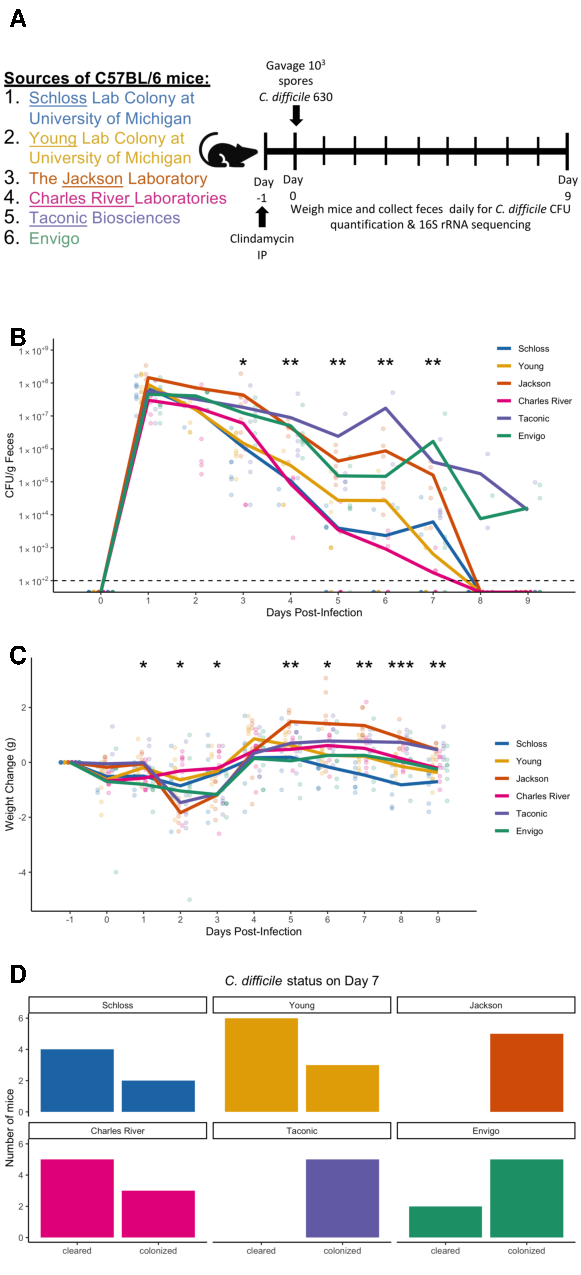
\includegraphics{figure_1.pdf} \textbf{Figure 1. Microbiota variation is
high between mice from different sources.} A-B. Number of observed OTUs
(A) and Shannon diversity index values (B) across sources of mice at
baseline (day -1 of the experiment). Differences between sources were
analyzed by Kruskal-Wallis test with Benjamini-Hochberg correction for
testing each day of the experiment and the adjusted \emph{P} value was
\textless{} 0.05 for panel A (Table S1). None of the \emph{P} values
from pairwise Wilcoxon comparisons between sources were significant
after Benjamini-Hochberg correction (Table S2). Gray lines represent the
median values for each source of mice. C. Principal Coordinates Analysis
(PCoA) of \(\theta_{YC}\) distances of baseline stool samples. Source
and the interaction between source and cage effects explained most of
the variation (PERMANOVA combined R\textsuperscript{2} = 0.90, \emph{P}
\textless{} 0.001, see Table S3). For A-C: each symbol represents the
value for a stool sample from an individual mouse, circles represent
experiment 1 mice and triangles represent experiment 2 mice. D. Plots
highlighting the median (point) and interquantile range (colored lines)
of the relative abundances for the top 20 bacteria out of the 268 OTUs
that varied across sources at baseline (Table S5).

\newpage

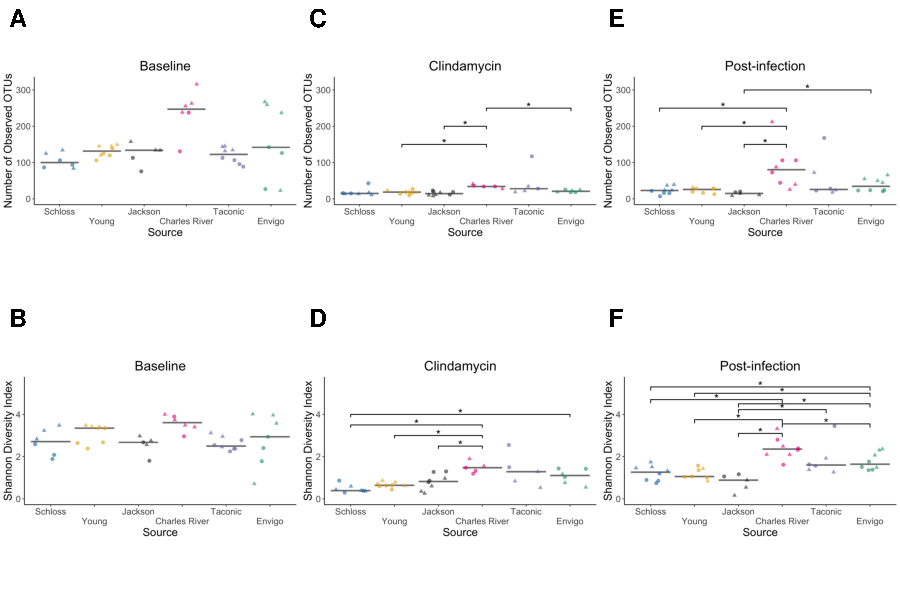
\includegraphics{figure_2.pdf}

\textbf{Figure 2. Clindamycin is sufficient to promote \emph{C.
difficile} colonization in all mice, but clearance time varies across
sources.} A. Setup of the experimental timeline. Mice for the
experiments were obtained from 6 different sources: the Schloss (N = 8)
and Young lab (N = 9) colonies at the University of Michigan, the
Jackson Laboratory (N = 8), Charles River Laboratory (N = 8), Taconic
Biosciences (N = 8), and Envigo (N = 8). All mice were administered 10
mg/kg clindamycin intraperitoneally (IP) 1 day before challenge with
\emph{C. difficile} 630 spores on day 0. Mice were weighed and feces was
collected daily through the end of the experiment (9 days
post-infection). Note: 3 mice died during course of experiment. 1
Taconic mouse prior to infection and 1 Jackson and 1 Envigo mouse
between 1- and 3-days post-infection. B. \emph{C. difficile} CFU/gram
stool measured over time (N = 20-49 mice per timepoint) via serial
dilutions. The black line represents the limit of detection for the
first serial dilution. CFU quantification data was not available for
each mouse due to early deaths, stool sampling difficulties, and not
plating all of the serial dilutions. C. Mouse weight change measured in
grams over time (N = 45-49 mice per timepoint), all mice were normalized
to the weight recorded 1 day before infection. For B-C: timepoints where
differences between sources of mice were statistically significant by
Kruskal-Wallis test with Benjamini-Hochberg correction for testing
across multiple days (Table S6 and Table S7) are reflected by the
asterisk above each timepoint (*, \emph{P} \textless{} 0.05). Lines
represent the median for each source and circles represent individual
mice from experiment 1 while triangles represent mice from experiment 2.

\newpage

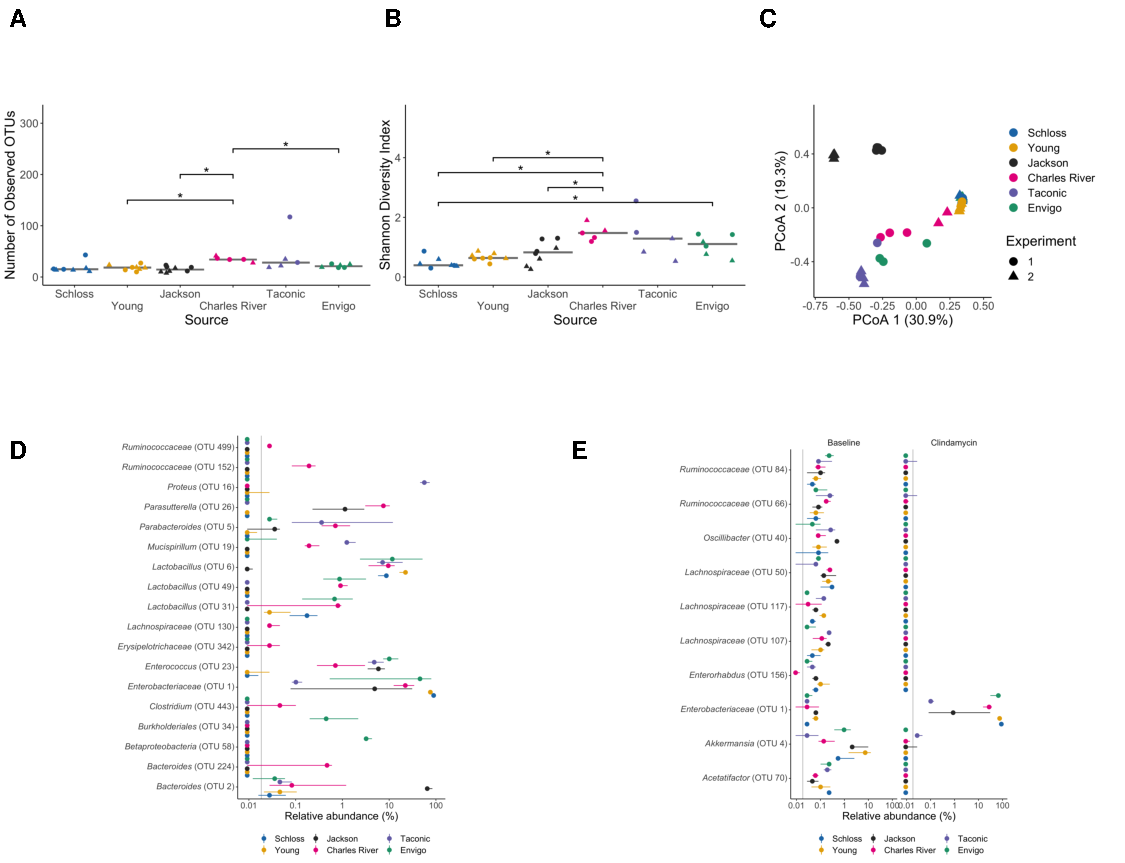
\includegraphics{figure_3.pdf} \textbf{Figure 3. Clindamycin treatment
alters bacteria in all sources, but a subset of bacterial differences
across sources persists.} A-B. Number of observed OTUs (A) and Shannon
diversity index values (B) across sources of mice after clindamycin
treatment (day 0). Differences between sources were analyzed by
Kruskal-Wallis test with Benjamini-Hochberg correction for testing each
day of the experiment and the adjusted \emph{P} value was \textless{}
0.05 (Table S1). Significant \emph{P} values from the pairwise Wilcoxon
comparisons between sources with Benjamini-Hochberg correction are shown
(Table S2). C. PCoA of \(\theta_{YC}\) distances from stools collected
post-clindamycin. Source and the interaction between source and cage
effects explained most of the variation observed post-clindamycin
(PERMANOVA combined R\textsuperscript{2} = 0.99, \emph{P} \textless{}
0.001, see Table S3). For A-C, each symbol represents a stool sample
from an individual mouse, with circles representing experiment 1 mice
and triangles representing experiment 2 mice. D. Plots highlighting the
median (point) and interquantile range (colored lines) of the relative
abundances for the 18 OTUs (Table S8)that varied between sources after
clindamycin treatment (day 0). E. Plots highlighting the median (point)
and interquantile range (colored lines) of the top 10 OTUs out of 153
with relative abundances that changed after clindamycin treatment
(adjusted \emph{P} value \textless{} 0.05). Data were analyzed by
Wilcoxon signed rank test of mice that had paired sequence data for
baseline (day -1) and post-clindamycin (day 0) timepoints (N = 31), with
Benjamini-Hochberg correction for testing all identified OTUs (Table
S9). The gray vertical line indicates the limit of detection.

\newpage

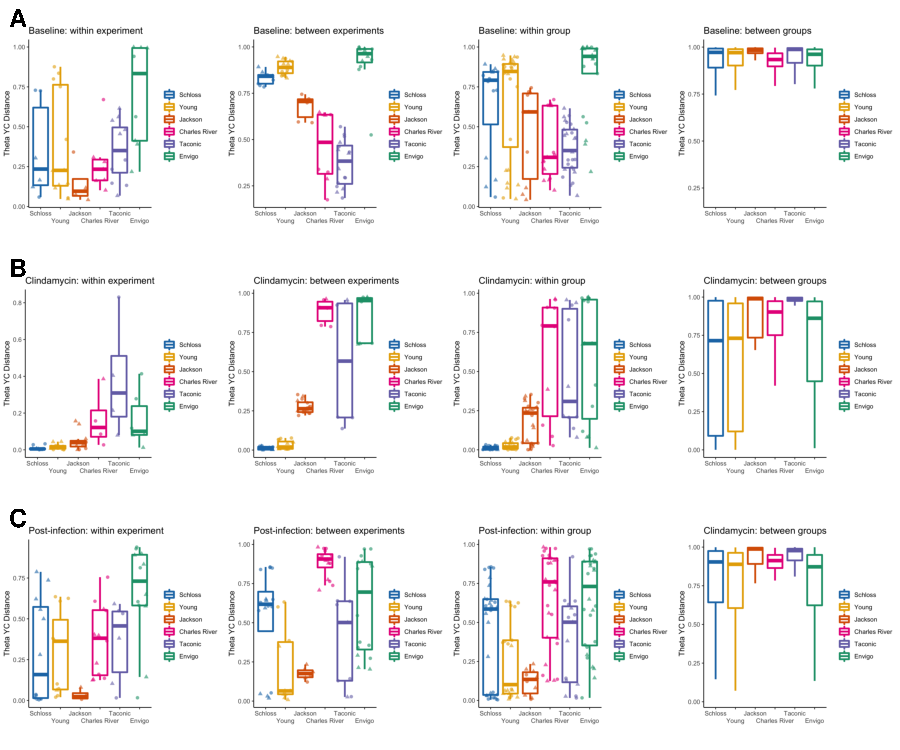
\includegraphics{figure_4.pdf} \textbf{Figure 4. Microbiota variation
across sources is maintained after \emph{C. difficile} challenge.} A-B.
Number of observed OTUs (A) and Shannon diversity index values (B)
across sources of mice 1-day post-infection. Data were analyzed by
Kruskal-Wallis test with Benjamini-Hochberg correction for testing each
day of the experiment and the adjusted \emph{P} value was \textless{}
0.05 (Table S1). Significant \emph{P} values from the pairwise Wilcoxon
comparisons between sources with Benjamini-Hochberg correction are shown
(Table S2). PCoA of \(\theta_{YC}\) distances of 1-day post-infection
stool samples. Source and the interaction between source and cage
effects explained most of the variation between fecal communities
(PERMANOVA combined R\textsuperscript{2} = 0.88, \emph{P} \textless{}
0.001, Table S3). For A-C: each symbol represents the value for a stool
sample from an individual mouse, circles represent experiment 1 mice and
triangles represent experiment 2 mice. D. Plots highlighting the median
(point) and interquantile range (colored lines) of the relative
abundances for the top 20 bacteria out of the 44 OTUs that varied
between sources 1-day post-infection. The gray vertical line indicates
the limit of detection. For each timepoint OTUs with differential
relative abundances across sources of mice were identified by
Kruskal-Wallis test with Benjamini-Hochberg correction for testing all
identified OTUs (Table S10). E. \(\theta_{YC}\) distances of fecal
samples collected 7-days post-infection relative to the baseline (day
-1) sample for each mouse. Each symbol represents an individual mouse.
Gray lines represent the median for each source.

\newpage

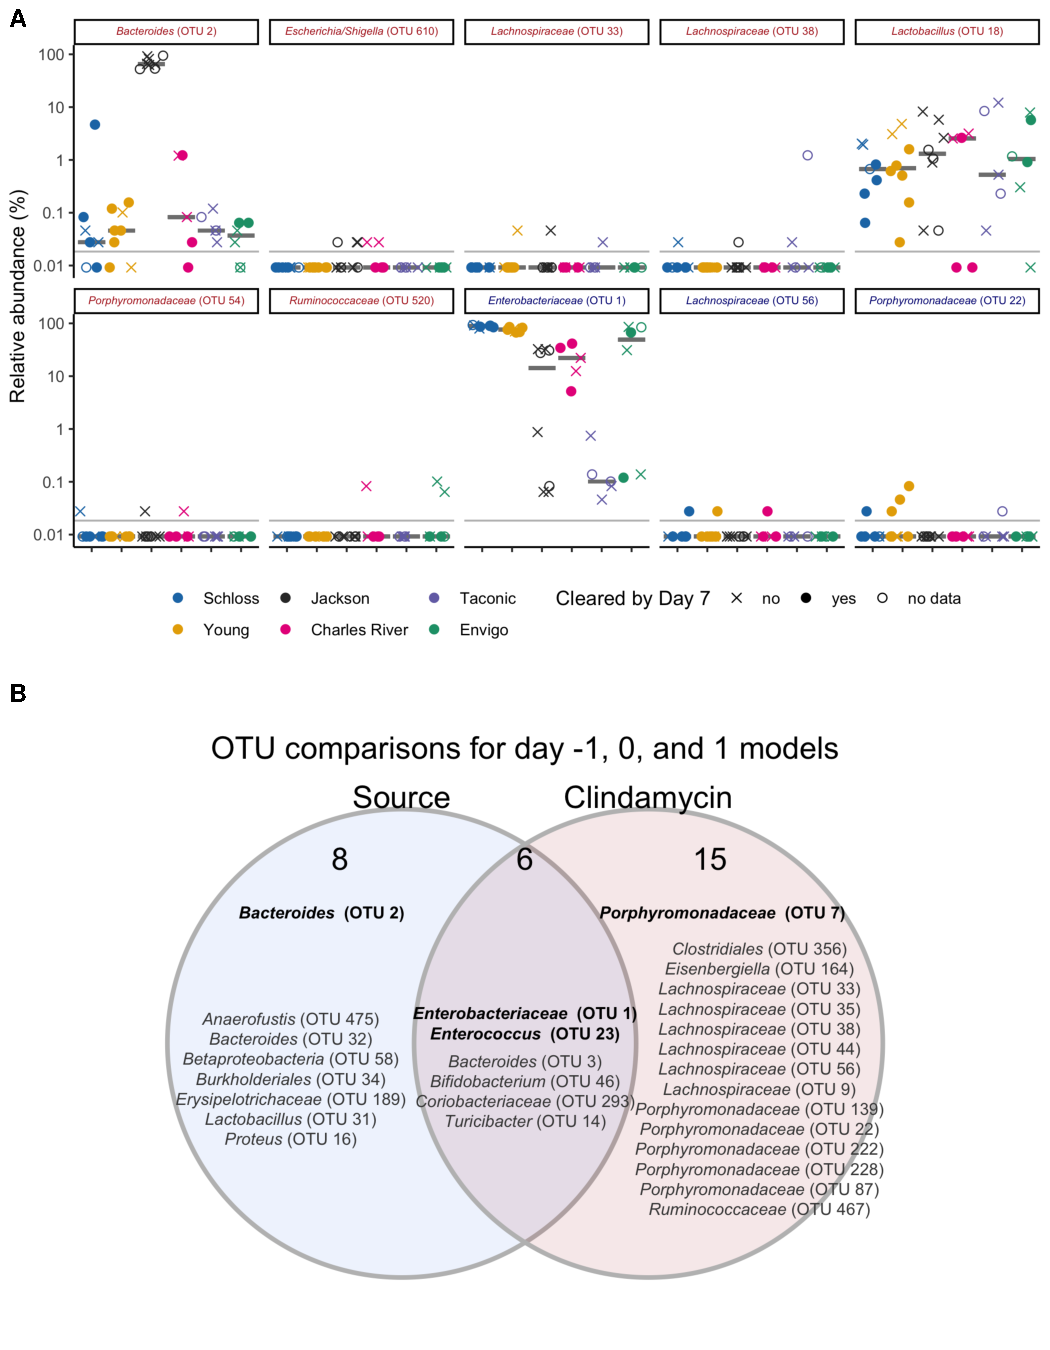
\includegraphics{figure_5.pdf} \textbf{Figure 5. Bacteria that influence
whether mice cleared \emph{C. difficile} by day 7.} A. Baseline (day 0)
relative abundance data for the 10 OTUs with the highest rankings based
on feature weights in the baseline (day 0) classification model. Red
font represents OTUs that correlated with \emph{C. difficile}
colonization and blue font represents OTUs that correlated with
clearance. Symbols represent the relative abundance data for an
individual mouse. Gray lines indicate the median relative abundances for
each source. B. Venn diagram that combines Fig. S4 summaries of OTUs
that were important to the day -1, 0, and 1 classification models (Table
S14) and either overlapped with taxa that varied across sources at the
same timepoint, were impacted by clindamycin treatment, or both. Red
OTUs were important to more than 1 classification model.

\newpage

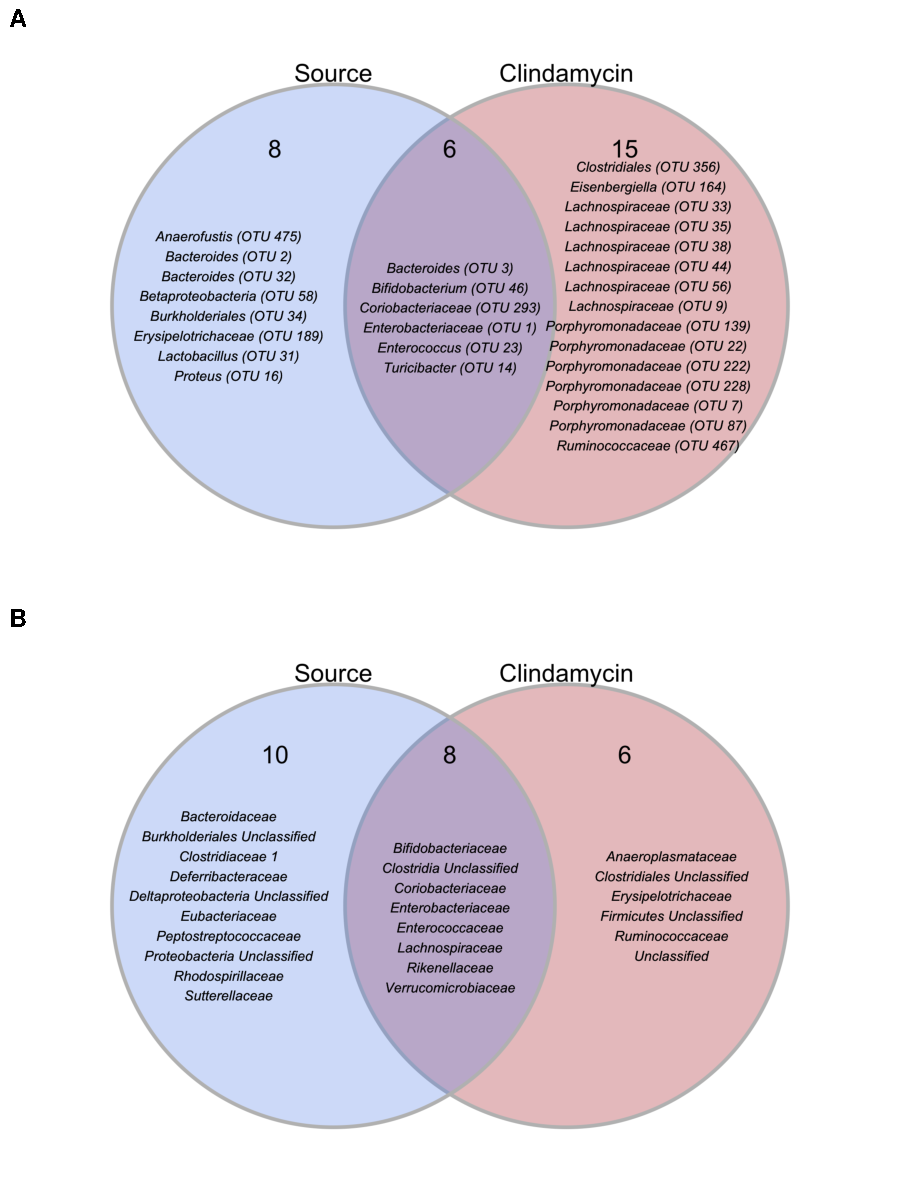
\includegraphics{figure_6.pdf} \textbf{Figure 6: OTUs associated with
\emph{C. difficile} colonization dynamics vary across sources throughout
the experiment.} A-D. Relative abundances of red OTUs from Fig. 5A that
were important for at least two classification models are shown over
time. A. \emph{Bacteroides} (OTU 2), which varied across sources
throughout the experiment. B-C. \emph{Enterobacteriaceae} (B) and
\emph{Enterococcus} (C), which significantly varied across sources and
were impacted by clindamycin treatment. D. \emph{Porphyromonadaceae}
(OTU 7), which was significantly impacted by clindamycin treatment and
after examining relative abundance dynamics over the course of the
experiment was found to also significantly vary between sources of mice
on days -1, 5, 6, 7, and 9 of the experiment. Symbols represent the
relative abundance data for an individual mouse. Colored lines indicate
the median relative abundances for each source. The gray horizontal line
represents the limit of detection. Timepoints where differences between
sources of mice were statistically significant by Kruskal-Wallis test
with Benjamini-Hochberg correction for testing across multiple days
(Table S15) are identified by the asterisk above each timepoint (*, P
\textless{} 0.05).

\newpage

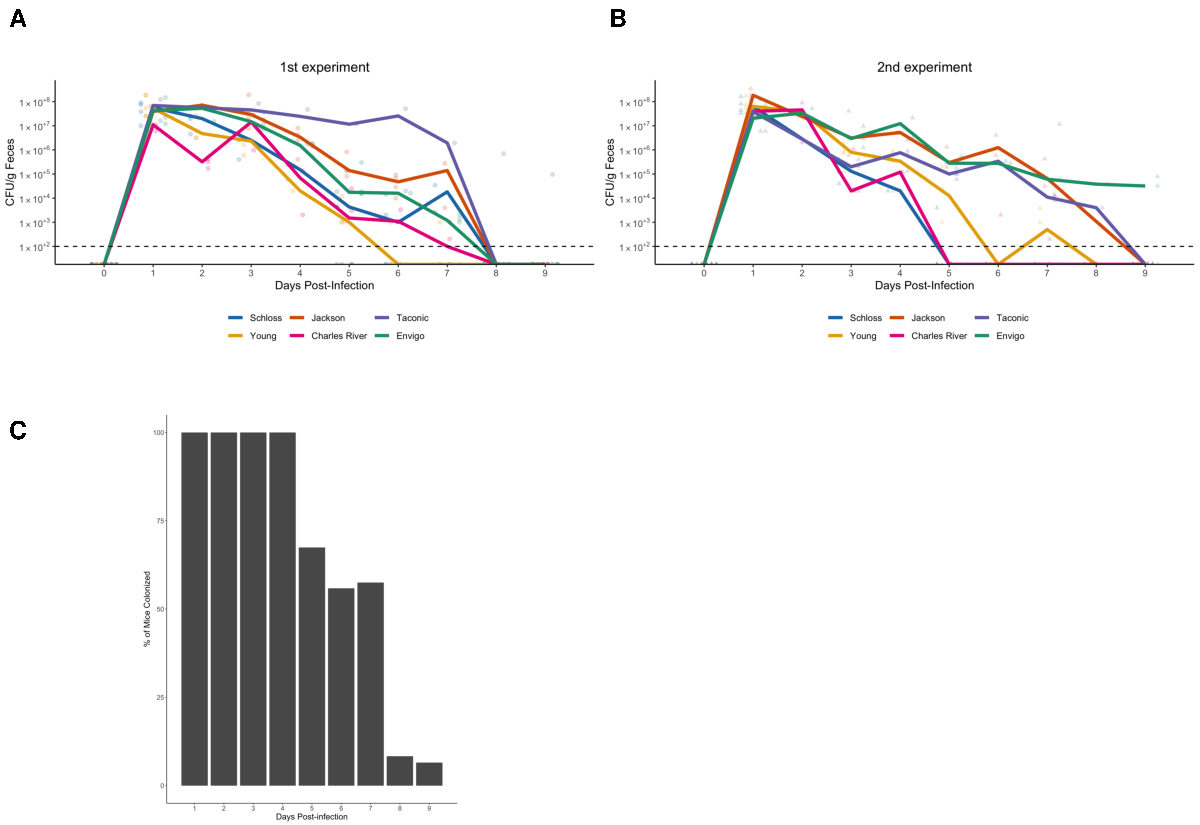
\includegraphics{figure_S1.pdf} \textbf{Figure S1. Bacterial communities
vary between experiments for some sources.} A-F. PCoA of \(\theta_{YC}\)
distances for the baseline fecal bacterial communities within each
source of mice. Each symbol represents a stool sample from an individual
mouse with color corresponding to experiment and shape representing cage
mates. Experiment number and cage effects explained most of the observed
variation for samples from the Schloss (PERMANOVA combined
R\textsuperscript{2} = 0.99; \emph{P} \(\le\) 0.033) and Young (combined
R\textsuperscript{2} = 0.95; \emph{P} \(\le\) 0.03) mice (Table S4).
G-H: Boxplots of the \(\theta_{YC}\) distances of the 6 sources of mice
relative to mice within the same source and experiment (G) or mice
within the same source and between experiments (H) at baseline (day -1).
Symbols represent individual mouse samples: circles for experiment 1 and
triangles for experiment 2.

\newpage

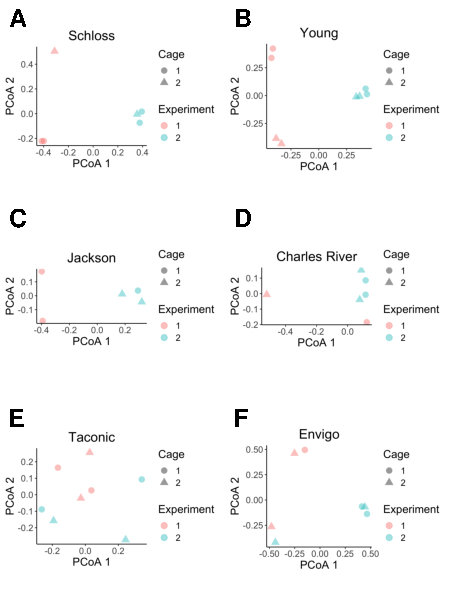
\includegraphics{figure_S2.pdf} \textbf{Figure S2. \emph{C. difficile}
CFU variation across sources varies slightly between the 2 experiments.}
A-B. \emph{C. difficile} CFU/gram of stool quantification over time for
experiment 1 (A) and 2 (B). Experiments were conducted approximately 3
months apart. Lines represent the median CFU for each source, symbols
represent individual mice and the black line represents the limit of
detection. C. \emph{C. difficile} CFU/gram stool 7-days post-infection
across sources of mice with an asterisk for pairwise Wilcoxon
comparisons with Benjamini-Hochberg correction where \emph{P}
\textless{} 0.05. D. Mouse weight change 2-days post-infection across
sources of mice, no pairwise Wilcoxon comparisons were significant after
Benjamini-Hochberg correction. For C-D: circles represent experiment 1
mice, triangles represent experiment 2 mice and gray lines indicate the
median values for each group. E. Percent of mice that were colonized
with \emph{C. difficile} over the course of the experiment. Each day the
percent is calculated based on the mice where \emph{C. difficile} CFU
was quantified for that particular day. Total N for each day: day 1 (N =
42), day 2 (N = 20), day 3 (N = 39), day 4 (N = 29), day 5 (N = 43), day
6 (N = 34), day 7 (N = 40), day 8 (N = 36), and day 9 (N = 46).

\newpage

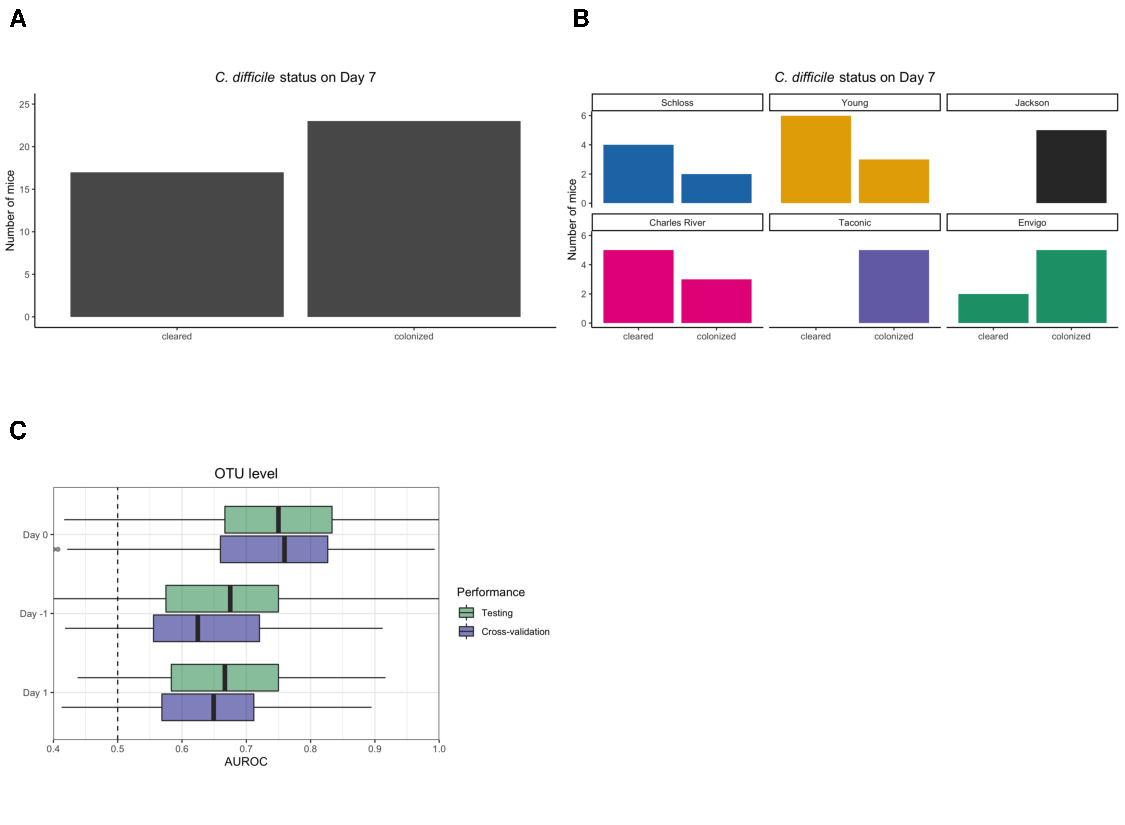
\includegraphics{figure_S3.pdf} \textbf{Figure S3. Bacterial community
composition before, after clindamycin perturbation, and post-infection
can predict \emph{C. difficile} colonization status 7 days
post-challenge.} A. Bar graph visualizations of overall 7-days
post-infection \emph{C. difficile} colonization status that were used as
classification outcomes to build L2-regularized logistic regression
models. Mice were classified as colonized or cleared (not detectable at
the limit of detection of 100 CFU) based on CFU g/stool data from 7 days
post-infection. B. \emph{C. difficile} CFU status on Day 7 within each
mouse source. N = 8-9 mice per group. C. L2-regularized logistic
regression classification model area under the receiving operator
characteristic curve (AUROCs) to predict \emph{C. difficile} CFU on day
7 post-infection (Fig. 2B, Fig. S2C) based on the OTU community relative
abundances at baseline (day -1), post-clindamycin (day 0), and 1-day
post-infection. All models performed better than random chance (AUROC =
0.5, all \emph{P} \(\le\) 1.6e-17, Table S12) and the model built with
post-clindamycin treated bacterial OTU relative abundances had the best
performance ((\emph{P}\textsubscript{FDR} \(\le\) 3.3e-06 for all
pairwise comparisons, Table S13). For list of the 20 OTUs that were
ranked as most important to each model, see Table S14.

\newpage

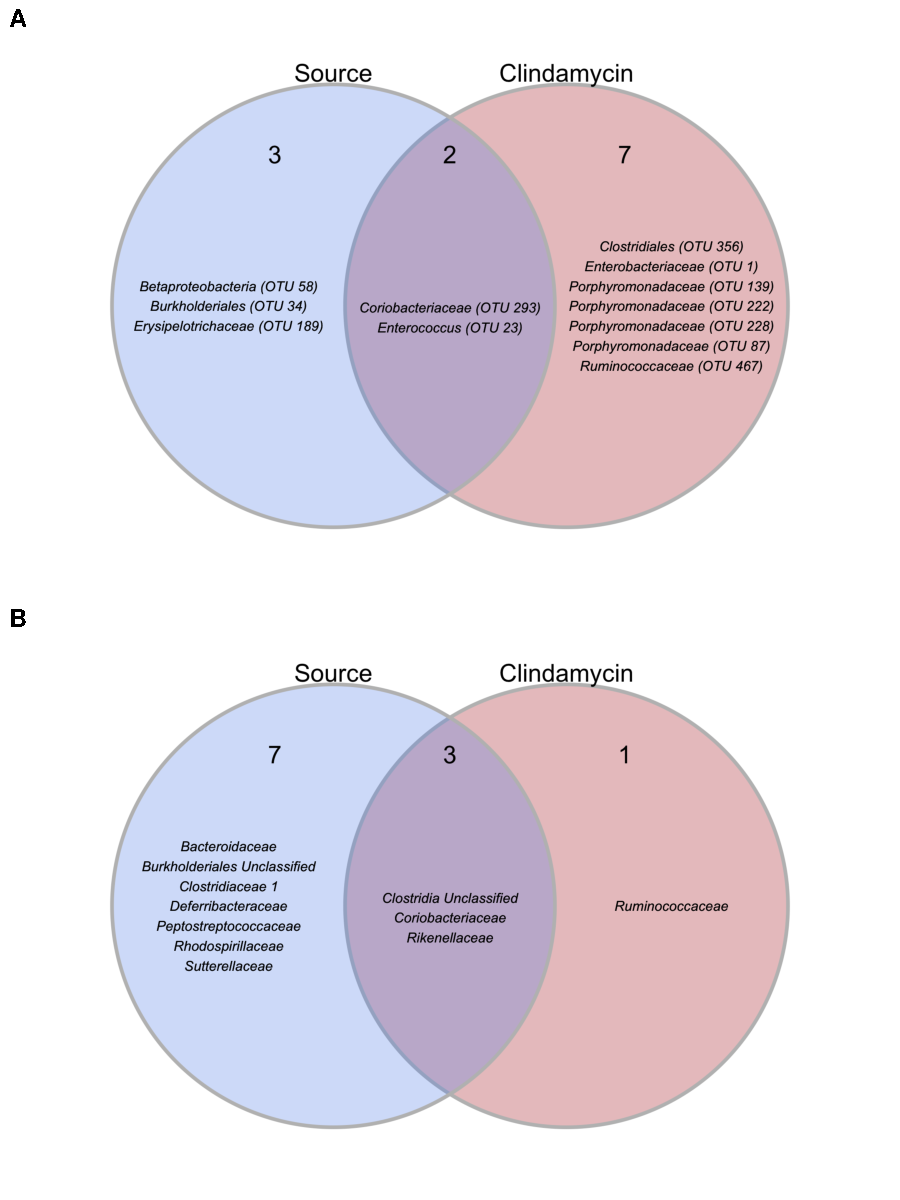
\includegraphics{figure_S4.pdf} \textbf{Figure S4. OTUs from
classification models based on baseline, post-clindamycin treatment, or
post-infection community data vary by source, clindamycin treatment, or
both.} A-C. Venn diagrams of OTUs from the top 20 OTUs from the baseline
(A), post-clindamycin treatment (B), and post-infection (C)
classification models (Table S14) that overlapped with OTUs that varied
across sources at the corresponding timepoint (Tables S5, 8, 10), were
impacted by clindamycin treatment (Table S9), or both. Red OTUs signify
OTUs that were important to more than 1 classification model.

\newpage

\hypertarget{supplementary-tables-and-movie}{%
\subsection{Supplementary Tables and
Movie}\label{supplementary-tables-and-movie}}

\textbf{Movie S1. Large shifts in bacterial community structure occurred
after clindamycin and \emph{C. difficile} infection.} PCoA of
\(\theta_{YC}\) distances animated from days -1 through 9 of the
experiment. Source was the variable that explained the most observed
variation across fecal communities (PERMANOVA source
R\textsuperscript{2} = 0.35, \emph{P} = 0.0001, Table S11) followed by
interactions between cage and day of the experiment. Transparency of the
symbol corresponds to the day of the experiment, each symbol represents
a sample from an individual mouse at a specific timepoint. Circles
represent mice from experiment 1 and triangles represent mice from
expeirment 2.

\textbf{Tables S1-S15. Excel workbook of Tables S1-S15.}

\textbf{Table S1. Alpha diversity metrics Kruskal-Wallis statistical
results.}

\textbf{Table S2. Alpha diversity metrics pairwise Wilcoxon statistical
results.}

\textbf{Table S3. PERMANOVA results for mice at baseline (day -1),
post-clindamycin (day 0), and post-infection (day 1).}

\textbf{Table S4. PERMANOVA results for each source of mice at baseline
(day -1).}

\textbf{Table S5. OTUs with relative abudances that significantly vary
between sources at baseline (day -1).}

\textbf{Table S6. \emph{C. difficile} CFU statistical results.}

\textbf{Table S7. Mouse weight change statistical results.}

\textbf{Table S8. OTUs with relative abudances that significantly vary
between sources post-clindamycin (day 0).}

\textbf{Table S9. OTUs with relative abudances that significantly
changed after clindamycin treatment.}

\textbf{Table S10. OTUs with relative abudances that significantly vary
between sources post-infection (day 1).}

\textbf{Table S11. PERMANOVA results for mice across all timepoints.}

\textbf{Table S12. Statistical results of L2-regularized logistic
regression model performances compared to random chance.}

\textbf{Table S13. Pairwise comparisons of L2-regularized logistic
regression model performances.}

\textbf{Table S14. Top 20 most important OTUs for each of the 3
L2-regularized logistic regression models based on OTU relative
abundance data.}

\textbf{Table S15. OTUs with relative abundances that significantly
varied across sources of mice on at least 1 day of the experiment by
Kruskal-Wallis test.}

\end{document}
